\section{Overview}%
\label{sec:chap3Overview}
\autoBookmark{sec}{Overview}
This chapter describes how the DAS event-classification artefact was designed, built, demonstrated, and evaluated. The artefact is a feature-driven pipeline that turns a raw DAS window into an event label through window-level conditioning, multi-domain feature engineering, ensemble feature selection, class-imbalance treatment, and lightweight classification. Every learning component runs on CPU cores, and the footprint of the whole pipeline, model size, latency, and training cost, is measured on the embedded platform on which it is meant to run. Its evaluation protocol is treated as part of the artefact rather than as neutral context: an accuracy that a deployment could not reproduce does not meet the design objectives, however good the individual components are.

The pipeline was designed on the Tomasov perimeter-security dataset, the primary dataset of the thesis, and then applied without modification to the Cao dataset, which serves as an independent evaluation dataset. Both datasets pass through every stage described below with the same settings. Where a stage has to treat them differently because their data are structured differently, the chapter says so explicitly.

The research follows the Design Science Research Methodology (DSRM) of Peffers et al.~\cite{peffers2007dsrm}. \refs{sec:chap3DSRMFramework} justifies that choice, presents the activity flow (\reff{fig:dsrm_flow}), and maps each research question and objective to a DSRM activity (Table~\ref{tab:dsrm_mapping}). \refs{sec:chap3DSRMProblem} to \refs{sec:chap3DSRMCommunication} then take the six activities in turn. Activity~3, the largest, contains the technical design: the datasets and how their samples are defined, the leakage found in their released protocols, the group-aware partitions that replace them, signal preprocessing, the extraction and fusion of $1{,}002$ features, the preparation of model-ready data, consensus feature selection and class balancing, classifier configuration, and the baseline models. Activity~4 describes the demonstration setting and the realised partitions. Activity~5 defines the metrics, the diagnostics, the statistical procedures, the generalisation tests, and the efficiency and lightweight-footprint measurements, and Activity~6 states how the results are communicated.

\section{Research Design: The DSRM Framework}
\label{sec:chap3DSRMFramework}
\autoBookmark{sec}{Research Design: The DSRM Framework}

\subsection{Rationale for Adopting DSRM}
\label{sec:chap3DSRMRationale}
\autoBookmark{subsec}{Rationale for Adopting DSRM}
Design science research produces and evaluates purposeful artefacts that address identified organisational or technical problems~\cite{hevner2004design}. Peffers et al.~\cite{peffers2007dsrm} operationalise this approach as a six-activity process with four possible entry points, and Gregor and Hevner~\cite{gregor2013positioning} classify the resulting knowledge contribution by the novelty of the problem and of the solution. DSRM suits the present study for three reasons. First, its principal output is a constructed artefact, a classification pipeline together with the protocol under which it is evaluated, rather than a description or explanation of a phenomenon. Second, the study is problem-centred: it starts from the operational limitations of DAS event classification (\refs{sec:ResearchProblemStatement}) and from a measurable deficiency in prevailing evaluation practice, and proceeds through design objectives and construction to assessment. Third, DSRM demands rigorous evaluation and the communication of reusable knowledge. Both demands are central here, because the most durable findings of the study concern how DAS benchmarks should be evaluated rather than which classifier wins on one of them. In Gregor and Hevner's terms, the evaluation protocol is an exaptation, known solutions carried into a field that had not applied them, and the pipeline with its diagnostics is an improvement, a new solution to a known problem (\refs{sec:chap5Contributions}).

DSRM has been applied to comparable machine-learning artefacts in engineering and information-systems research, where the artefact is a data pipeline or predictive system whose utility is established empirically. Its activities align with the three research questions of \refs{sec:ResearchQuestions}: RQ1 analyses the footprint a lightweight classifier must meet and so shapes the problem and the objectives; RQ2 guides the design and development of the pipeline and its components; and RQ3 evaluates it under a verified leakage-controlled protocol, benchmarks it against alternatives, and tests how far its performance generalises.

\subsection{DSRM Activity Flow}
\label{sec:chap3DSRMFlow}
\autoBookmark{subsec}{DSRM Activity Flow}
\reff{fig:dsrm_flow} shows the six activities as executed in this study, with the entry point, the input each activity received, the output it produced, and the section in which it is documented. The process was iterative, as Peffers et al.\ anticipate, and evidence from Activity~5 fed back into Activity~3 on three occasions. The first blocked partition of the Tomasov data balanced zone counts rather than window mass, left one class with no test samples, and was redesigned. The Friedman analysis first used to compare classifiers was withdrawn once its blocking assumption was found to be violated, and was replaced by tests over independent acquisitions. The set of baselines was widened from the two published CNNs to five architectures published from 2024 onwards. Every refinement was decided on training and validation evidence; the held-out test sets were not consulted until the final evaluation.

\begin{figure}[!htbp]
\centering
\begin{tikzpicture}[
	font=\footnotesize,
	node distance=3mm and 5mm,
	act/.style={draw, thick, rounded corners=2pt, fill=gray!15, text width=3.2cm, align=center, inner sep=4pt},
	io/.style={draw, fill=white, text width=8.6cm, align=left, inner sep=4pt},
	ref/.style={font=\scriptsize\itshape},
	arr/.style={-{Latex[length=2.2mm]}, thick},
	iter/.style={-{Latex[length=2.2mm]}, thick, dashed},
]
\node[io] (o1) {\textbf{In:} research gaps from the literature (Chapter~\ref{chap:LR}); leakage audit of the released evaluation protocols.\\\textbf{Out:} problem statement; research questions RQ1--RQ3.\\{\scriptsize\itshape \refs{sec:chap3DSRMProblem}}};
\node[io, below=of o1] (o2) {\textbf{In:} RQ1--RQ3.\\\textbf{Out:} research objectives RO1--RO3; six design criteria including evaluative validity.\\{\scriptsize\itshape \refs{sec:chap3DSRMObjectives}}};
\node[io, below=of o2] (o3) {\textbf{In:} primary (Tomasov) and evaluation (Cao) datasets; design criteria.\\\textbf{Out:} verified group-aware partitions; stateless preprocessing chain; $1{,}002$-feature extractor; eight-method consensus selection; six balancing strategies; seven classifiers; published-CNN and recent-architecture baselines.\\{\scriptsize\itshape \refs{sec:chap3DSRMDesign}}};
\node[io, below=of o3] (o4) {\textbf{In:} artefact; frozen partition manifests; Jetson AGX Orin.\\\textbf{Out:} trained configurations on both datasets for the full and consensus feature sets; baselines trained on identical partitions.\\{\scriptsize\itshape \refs{sec:chap3DSRMDemonstration}}};
\node[io, below=of o4] (o5) {\textbf{In:} predictions on the held-out test partitions.\\\textbf{Out:} effectiveness and per-class behaviour; confound and protocol-attribution diagnostics; generalisation across recordings, campaigns, and systems, including the Tomasov--Cao label mapping; statistics over independent acquisitions; efficiency.\\{\scriptsize\itshape \refs{sec:chap3DSRMEvaluation}; Chapter~\ref{chap:ResultsAndDiscussion}}};
\node[io, below=of o5] (o6) {\textbf{Out:} this thesis; journal and conference publications; public code, partition manifests, predictions, and assumption files.\\{\scriptsize\itshape \refs{sec:chap3DSRMCommunication}; Chapter~\ref{chap:Conclusion}}};

\node[act, left=of o1] (a1) {\textbf{Activity 1}\\Problem identification and motivation};
\node[act, left=of o2] (a2) {\textbf{Activity 2}\\Objectives of a solution};
\node[act, left=of o3] (a3) {\textbf{Activity 3}\\Design and development};
\node[act, left=of o4] (a4) {\textbf{Activity 4}\\Demonstration};
\node[act, left=of o5] (a5) {\textbf{Activity 5}\\Evaluation};
\node[act, left=of o6] (a6) {\textbf{Activity 6}\\Communication};
\node[draw, dashed, rounded corners=2pt, above=4mm of a1, text width=3.2cm, align=center, inner sep=3pt] (entry) {Problem-centred initiation};

\draw[arr] (entry) -- (a1);
\draw[arr] (a1) -- (a2);
\draw[arr] (a2) -- (a3);
\draw[arr] (a3) -- (a4);
\draw[arr] (a4) -- (a5);
\draw[arr] (a5) -- (a6);
\foreach \i in {1,...,6} {\draw[arr] (a\i) -- (o\i);}
\draw[iter] (a5.west) -- ++(-0.5,0) |- node[pos=0.25, left, ref] {refine} (a3.west);
\end{tikzpicture}
\caption{DSRM activity flow followed in this study, adapted from Peffers et al.~\cite{peffers2007dsrm}. Each activity lists its principal inputs and outputs and the section in which it is reported. The dashed return path marks the design refinements triggered by evaluation evidence.}
\label{fig:dsrm_flow}
\end{figure}

\subsection{Mapping of Research Questions, Objectives, and Activities}
\label{sec:chap3DSRMMapping}
\autoBookmark{subsec}{Mapping of Research Questions, Objectives, and Activities}
Table~\ref{tab:dsrm_mapping} maps each research question to its objective and DSRM activities. It is the contract against which Chapter~\ref{chap:Conclusion} judges whether each objective was met. RO1 is analytical: it draws on the review of Chapter~\ref{chap:LR} to set the lightweight requirement in Activities~1 and~2, and on the footprint measurements of Activity~5 to check it. RO2 is constructive and is met by the artefact built in Activity~3 and run in Activity~4. RO3 is evaluative. It includes the design of the leakage-controlled partitions in Activity~3, since a protocol that has not been verified cannot support an evaluation.

\begin{table}[!htbp]
\centering
\caption{Mapping of research questions, research objectives, and DSRM activities.}
\label{tab:dsrm_mapping}
\footnotesize
\setlength{\tabcolsep}{4pt}
\renewcommand{\arraystretch}{1.2}
\begin{tabularx}{\textwidth}{@{}>{\raggedright\arraybackslash}X >{\raggedright\arraybackslash}X >{\raggedright\arraybackslash}p{2.4cm}@{}}
\toprule
\textbf{Research question} & \textbf{Research objective} & \textbf{DSRM activity}\\
\midrule
\textbf{RQ1.} What computational footprint do current approaches to event classification in DAS data carry, and what makes a classification pipeline lightweight? &
\textbf{RO1.} To analyse the computational footprint of event classification in Distributed Acoustic Sensing data and establish what makes a classification pipeline lightweight. &
1 (problem), 2 (objectives), 5 (evaluation)\\
\addlinespace
\textbf{RQ2.} How can multi-domain fusion, consensus feature selection, and class balancing be combined into a lightweight pipeline for event classification in DAS data? &
\textbf{RO2.} To develop a multi-domain machine learning pipeline for event classification in Distributed Acoustic Sensing data. &
3 (design), 4 (demonstration)\\
\addlinespace
\textbf{RQ3.} How does the pipeline compare with published deep-learning baselines on identical leakage-controlled partitions in classification performance, computational cost, and generalisation? &
\textbf{RO3.} To evaluate the multi-domain machine learning pipeline for event classification in Distributed Acoustic Sensing data. &
3 (design), 4 (demonstration), 5 (evaluation)\\
\bottomrule
\end{tabularx}
\end{table}

\section{DSRM Activity 1: Problem Identification and Motivation}
\label{sec:chap3DSRMProblem}
\autoBookmark{sec}{DSRM Activity 1: Problem Identification and Motivation}
The first activity establishes the practical problem that the artefact must solve. \refs{sec:ResearchProblemStatement} set out the established difficulties: raw DAS streams are noisy and high-dimensional, engineered feature sets are redundant and costly to compute, class imbalance is severe, and the deep models that lead on accuracy are expensive to run on edge hardware. These difficulties defined the initial aim of the research, a feature-driven pipeline that is accurate, interpretable, and cheap enough to run alongside the interrogator. Analysing what ``cheap enough'' means (RO1) showed that the literature offers no common measure of it: where cost is reported it is usually an inference time, which says nothing about how large the model is, what hardware trains it, or how long its input takes to prepare (\refs{sec:chap2ResearchGap}). The lightweight requirement therefore had to be defined before it could be designed for.

A further problem emerged as the work progressed. The pipeline was first evaluated on the Tomasov dataset alone, and extending it to the Cao dataset required its evaluation protocol to be specified for data with a different structure. Doing so showed that the protocols used with both datasets allow information to pass between training and test data. The mechanism is structural. DAS event datasets are built by sliding a window along a continuous stream, so neighbouring windows share raw samples whenever the hop is shorter than the window, and every window from one recording session shares the fibre state, coupling, interrogator settings, weather, and often the operator. A partition that ignores this dependence measures how well a model recognises a recording it has already seen, which is not the quantity that matters in deployment. \refss{sec:chap3LeakageAudit} describes how the problem was identified and shows that it is real: 423 of 441 Cao sessions span the released partition, and every test window of a random Tomasov split shares raw samples with a training window. Because a published accuracy obtained under such a protocol mixes the method with the protocol, verified leakage-controlled partitions became part of the artefact and the evaluation basis for all three research questions.

\section{DSRM Activity 2: Objectives of a Solution}
\label{sec:chap3DSRMObjectives}
\autoBookmark{sec}{DSRM Activity 2: Objectives of a Solution}
The second activity translates the problem into objectives. In line with RO1 to RO3 (\refs{sec:ResearchObjectives}), the artefact must (i) meet a lightweight footprint defined by measured quantities, (ii) classify DAS events interpretably through multi-domain fusion, consensus selection, and class balancing whose effects are exposed, and (iii) withstand comparison with published baselines on identical, verified leakage-controlled partitions.

Six design criteria follow from these objectives. \emph{Effectiveness} is measured by macro-$F_1$ and balanced accuracy on held-out data. \emph{Lightweight footprint} is measured by four quantities on embedded hardware: the stored size of the trained model, per-window inference latency, per-window end-to-end latency including feature extraction, and training time together with the hardware it needs. The target is CPU-only training and inference, a model of a few megabytes, sub-millisecond classification, and an online cost that fits the window-arrival interval on a few CPU cores. Of the remaining criteria, \emph{interpretability} is measured by the traceability of every selected feature to a named descriptor and signal domain; \emph{robustness} by stability under class imbalance, repeated partitioning, and held-out acquisitions; and \emph{reproducibility} by fixed seeds, frozen partition manifests, and released code. The sixth criterion, \emph{evaluative validity}, is the property that a reported metric is measured under conditions a deployment could reproduce. It is the criterion that distinguishes this design cycle from earlier work on the same benchmarks, and it is enforced by assertions in code rather than by statements in text.

\section{DSRM Activity 3: Design and Development}
\label{sec:chap3DSRMDesign}
\autoBookmark{sec}{DSRM Activity 3: Design and Development}
The artefact is an end-to-end, feature-driven pipeline built in six phases, each documented in its own subsection: data acquisition, leakage identification, and partitioning (\refss{sec:chap3Phase1}); signal preprocessing (\refss{sec:chap3Preprocessing}); multi-domain feature extraction and fusion (\refss{sec:chap3Phase2}); preparation of model-ready data (\refss{sec:chap3ModelReady}); feature selection and class balancing (\refss{sec:chap3Phase3}); and classifier design (\refss{sec:chap3Phase4}). The baselines against which the artefact is compared, two published CNNs and five recent architectures, are described in \refss{sec:chap3Baselines}. \reff{fig:methodology_framework} draws the complete workflow as a flowchart with standard symbols, from the two datasets through partitioning, the feature pipeline, and the baseline branch to evaluation. Every phase runs on the primary Tomasov dataset and then, unchanged, on the Cao evaluation dataset; the few steps that must differ between them are marked in the figure. Its two decision points mark where the workflow branches or loops: a partition that fails verification is redesigned, and models are trained both with and without feature selection, with the validation set guiding the choice of balancing strategy, classifier, and hyperparameters. The order of the workflow is itself a control: the leakage audit and the group-aware partition come first, before any signal is processed, and every component that learns from data (feature selection, resampling, and feature scaling) is fitted on training rows only.

\clearpage
\begin{figure}[p]
\centering
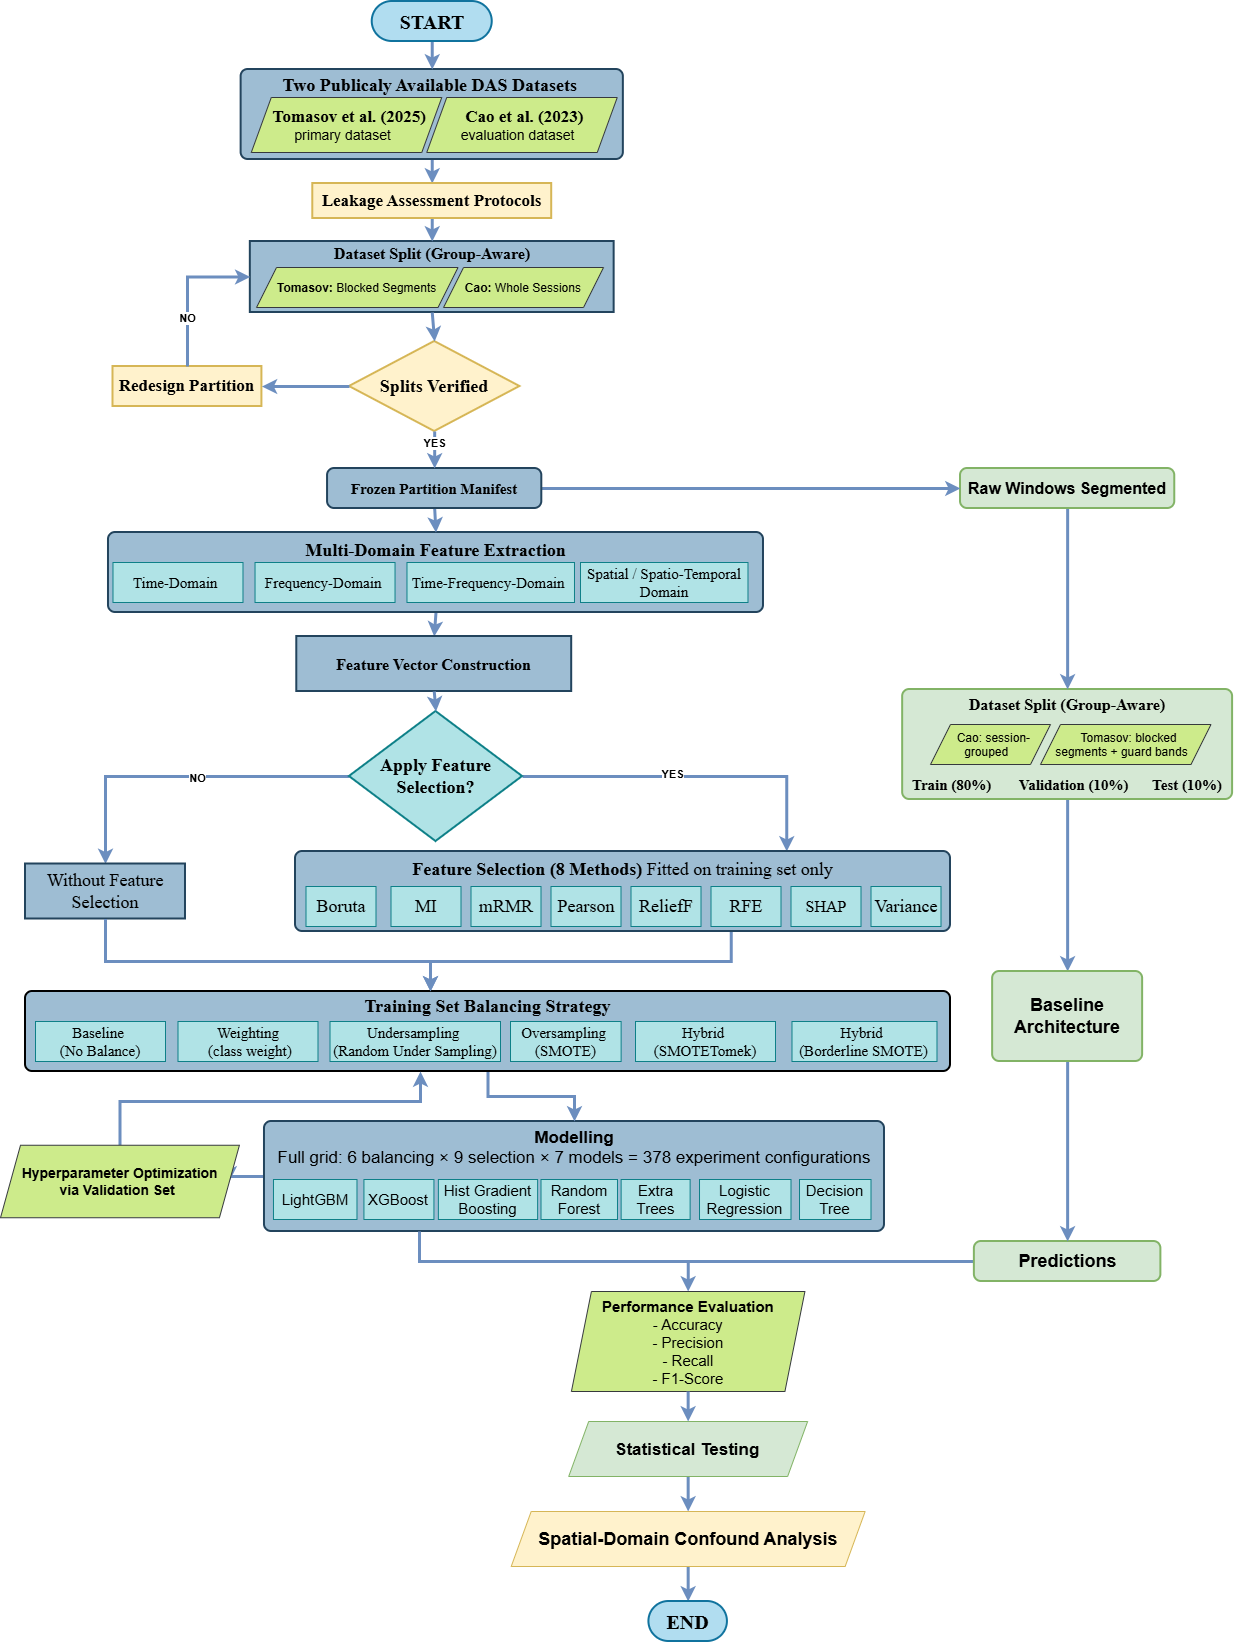
\includegraphics[width=\textwidth,height=0.80\textheight,keepaspectratio]{Figures/fig03_EC_pineline.png}
\caption[Complete workflow of the study]{Complete workflow of the study. Tomasov (primary) and Cao (evaluation) pass through the same pipeline; the branch on the right trains the baseline architectures on raw windows from the same group-aware partitions.}
\label{fig:methodology_framework}
\end{figure}
\clearpage

\subsection{Data Acquisition, Leakage Identification, and Partitioning}
\label{sec:chap3Phase1}
\autoBookmark{subsec}{Data Acquisition, Leakage Identification, and Partitioning}

\subsubsection{Dataset Description}
\label{sec:chap3Dataset}
\autoBookmark{subsubsec}{Dataset Description}
Two public DAS datasets are used, with distinct roles. The Tomasov perimeter-security dataset~\cite{tomasov2025dataset} is the primary dataset: the pipeline was designed on it, and it carries the main results. The Cao dataset~\cite{caoxin2023opendataset} is the evaluation dataset, used to test whether the design and its conclusions hold on an independent acquisition system. The two share no hardware, sensing principle, channel geometry, or event taxonomy, and that is the point of using both: a conclusion that holds on each can be attributed to the method rather than to one installation. They also arrive in different forms. Tomasov is released as continuous interrogator streams with hand-drawn annotations and no partition, whereas Cao is released as pre-segmented records already divided into fixed training and test folders. This difference governs how each is turned into labelled samples (\refss{sec:chap3Manifests}) and how its dependence structure must be controlled (\refss{sec:chap3Partitioning}). Table~\ref{tab:dataset_comparison} summarises both.

\begin{table}[!htbp]
	\centering
	\caption{The two public DAS datasets used in this study.}
	\label{tab:dataset_comparison}
	\small
	\begin{tabular}{@{}lll@{}}
		\toprule
		\textbf{Property} & \textbf{Tomasov \etal\ 2025} & \textbf{Cao \etal\ 2023}\\
		\midrule
		Role in this study  & Primary dataset            & Evaluation dataset \\
		Sensing principle   & Phase-sensitive OTDR       & Intensity $\Phi$-OTDR \\
		Interrogator        & OptaSense ODH-F            & Not specified \\
		Event classes       & 9                          & 6 \\
		Spatial channels    & 1{,}700                    & 12 \\
		Channel spacing     & 1.02\,m                    & 10\,m \\
		Sampling rate       & 20\,kHz                    & 8--12.5\,kHz (nominal) \\
		Sample unit         & Continuous stream          & Pre-segmented record \\
		Analysis windows    & 439{,}754                  & 15{,}418 \\
		Independent groups  & 16 recordings              & 441 sessions \\
		Imbalance (max:min) & 30.9:1                     & 1.3:1 \\
		\bottomrule
	\end{tabular}
\end{table}

\paragraph[Tomasov \etal\ (2025): Primary Dataset]{Tomasov \etal\ (2025): Primary Dataset.}
The perimeter-security dataset~\cite{tomasov2025dataset} was acquired with an OptaSense ODH-F interrogator on a university campus, with the fibre buried about 1\,m beneath the pavement, and is released as HDF5 files. The interrogator samples $1{,}700$ loci at 1.02\,m spacing with a 20\,kHz pulse rate. Nine event classes were annotated by hand on band-limited power maps and distributed as a Boolean mask over (time-block, locus) cells. Applying the published $8{,}192$-sample window with a $2{,}048$-sample hop yields $439{,}754$ annotated windows across 16 recordings. \reff{fig:campus_map} shows the campus layout and label points, and Table~\ref{tab:dataset} and \reff{fig:tomasov_counts} give the class-wise statistics.

\paragraph[Cao \etal\ (2023): Evaluation Dataset]{Cao \etal\ (2023): Evaluation Dataset.}
The intensity-based $\Phi$-OTDR release~\cite{caoxin2023opendataset} contains six event classes as $15{,}419$ pre-segmented MATLAB records of $10{,}000$ time samples across 12 adjacent spatial points at 10\,m spacing. Two fibre spans (5.1\,km and 10.1\,km) were used, so the same $10{,}000$ samples cover either 0.8\,s or 1.25\,s; the release carries no per-file marker distinguishing them, so a nominal sampling rate is adopted and recorded as an assumption. One zero-byte record in the released test folder, belonging to the background class, is excluded, leaving $15{,}418$ usable records: background $2{,}945$, digging $2{,}512$, knocking $2{,}530$, watering $2{,}253$, shaking $2{,}728$, and walking $2{,}450$.

\begin{table}[!htbp]
	\centering
	\caption{Class-wise statistics of the Tomasov perimeter-security dataset.}
	\label{tab:dataset}
	\small
	\begin{tabular}{@{}lrrr@{}}
		\toprule
		\textbf{Class} & \textbf{Windows} & \textbf{Recordings} & \textbf{Share (\%)}\\
		\midrule
		Regular      & 210{,}023 & 1 & 47.76\\
		Car          & 58{,}017  & 4 & 13.19\\
		Construction & 54{,}832  & 1 & 12.47\\
		Fence        & 43{,}981  & 3 & 10.00\\
		Walk         & 19{,}155  & 2 & 4.36\\
		Manipulation & 17{,}710  & 1 & 4.03\\
		Longboard    & 15{,}367  & 2 & 3.49\\
		Running      & 13{,}877  & 1 & 3.16\\
		Openclose    & 6{,}792   & 1 & 1.54\\
		\bottomrule
	\end{tabular}
\end{table}

\begin{figure}[!htbp]
\centering
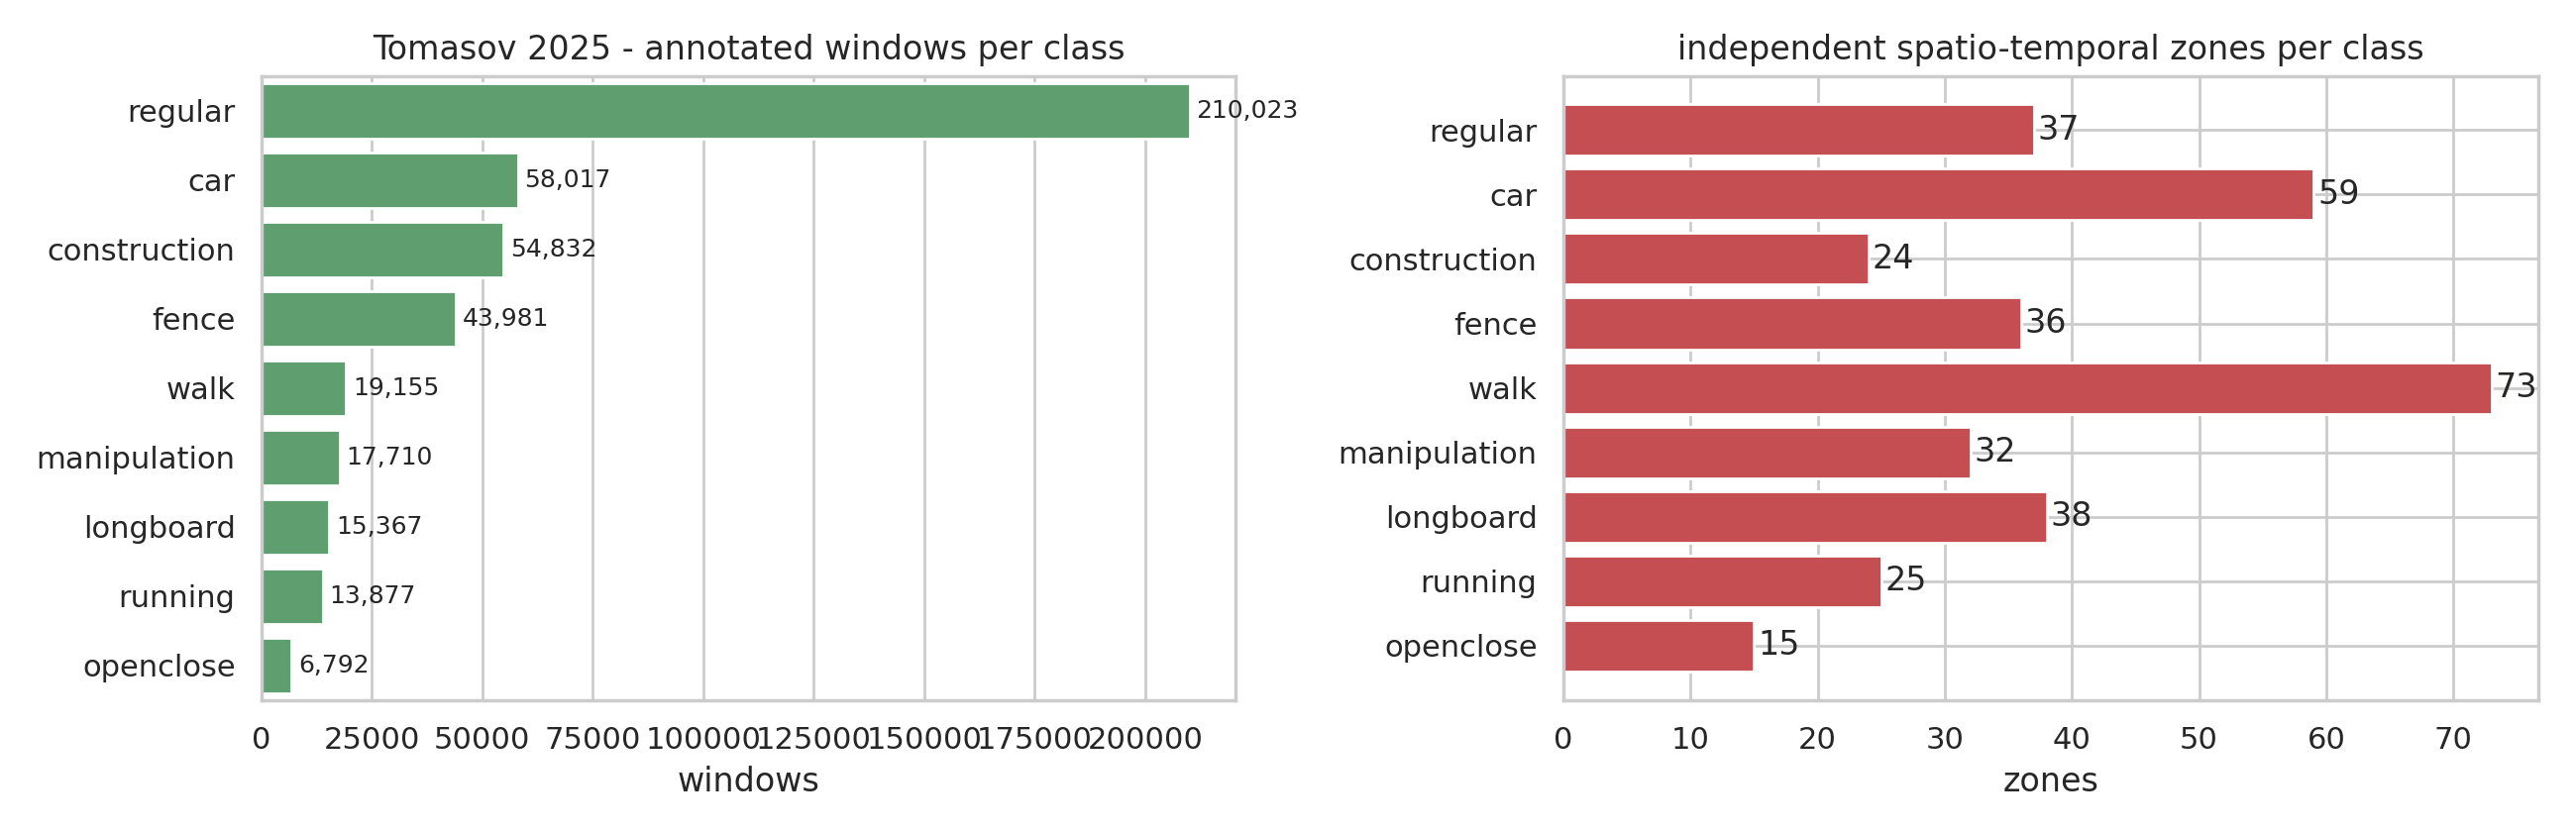
\includegraphics[width=0.95\textwidth,keepaspectratio]{Figures/fig27_tomasov_class_zone_counts.png}
\caption{Tomasov dataset inventory: annotated windows per class (left) and independent spatio-temporal zones per class (right). The zone count is the number of contiguous annotated regions and bounds how many independent groups any partition can draw on.}
\label{fig:tomasov_counts}
\end{figure}

Table~\ref{tab:dataset} records a fact that governs the whole analysis. Five of the nine Tomasov classes (\emph{construction}, \emph{manipulation}, \emph{openclose}, \emph{regular}, and \emph{running}) come from exactly one recording each, so for those classes recording identity and class identity are the same variable. No partition of this dataset can separate them; \refss{sec:chap3ConfoundDesign} describes the diagnostic designed to measure the consequence rather than assume it away.

\begin{figure}[!htbp]
\centering
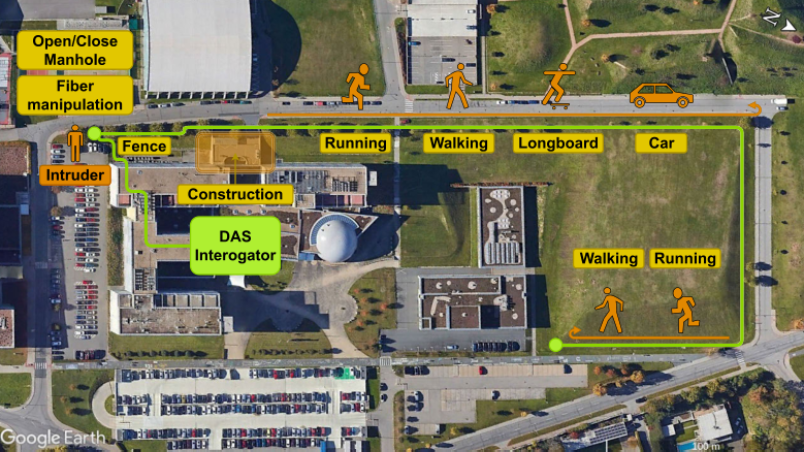
\includegraphics[width=0.85\textwidth]{Figures/fig04_campus_map.png}
\caption{Perimeter-security DAS setup and event labels along the monitored fibre path.}
\label{fig:campus_map}
\end{figure}

\subsubsection{Construction of Sample Manifests}
\label{sec:chap3Manifests}
\autoBookmark{subsubsec}{Construction of Sample Manifests}
Before any signal is read, each dataset is converted into a \emph{sample manifest}: a table with one row per analysis window that records the window's class label, its physical provenance, and the identifiers of every dependence group to which it belongs. The manifest is built from metadata alone (the annotation masks and the filenames), so it can be constructed, audited, and partitioned in seconds without loading the raw interrogator data. Every later stage, from feature extraction to final evaluation, is joined to the manifest through a unique sample identifier, which makes the manifest the single authoritative record of what each sample is and where it came from. Table~\ref{tab:manifest} lists the fields recorded for each dataset.

For Tomasov, labels are derived from the released annotation mask, a Boolean array over (time-block, locus) cells in which one block spans $H = 2{,}048$ raw samples. Each annotated cell whose block index $b$ leaves room for a complete window, $b \le n_{\mathrm{blocks}} - L/H$, becomes one manifest row, labelled with the event class of the recording in which it lies. The row stores the recording identifier, the block index, the locus, and the raw-sample interval $[bH,\, bH + L)$ that the window will read. Recording this interval explicitly is what later allows the leakage audit and the guard bands to be computed exactly rather than approximately. Acquisition parameters are read from the attributes of each HDF5 file rather than assumed, and all 16 recordings were confirmed to share a 20\,kHz pulse rate and $1{,}700$ loci. Because the annotations mark many loci within each block, the manifest is dense in space as well as in time: the \emph{regular} recording alone contributes $210{,}023$ windows drawn from 738 blocks and 622 loci.

For Cao, each \texttt{.mat} record becomes one manifest row, labelled by the class folder in which it is stored. The filename is parsed into acquisition date, operator, event token, session token, and record index, and the session identifier concatenates date, operator, class, and session token, because a session token is unique only within that combination. The acquisition date is kept separately as the grouping unit for the leave-one-date-out evaluation of \refss{sec:chap3ConfoundDesign}. The released folder, training or test, is also recorded, but only so that the released protocol can be audited; it plays no part in the partition used in this study. The zero-byte record noted in \refss{sec:chap3Dataset} is flagged at this stage and excluded, leaving $15{,}418$ rows.

\begin{table}[!htbp]
	\centering
	\caption{Contents of the sample manifests. The Tomasov split group is assigned during partitioning (\refss{sec:chap3Partitioning}); every other field is derived from the released metadata.}
	\label{tab:manifest}
	\small
	\setlength{\tabcolsep}{4pt}
	\begin{tabularx}{\textwidth}{@{}>{\raggedright\arraybackslash}p{2.7cm} >{\raggedright\arraybackslash}X >{\raggedright\arraybackslash}X@{}}
		\toprule
		\textbf{Field} & \textbf{Tomasov \etal\ 2025} & \textbf{Cao \etal\ 2023}\\
		\midrule
		Unit (one row)   & One annotated (time-block, locus) cell & One pre-segmented \texttt{.mat} record\\
		Label source     & Event class of the annotated recording & Class folder of the record\\
		Provenance       & Recording, block index, locus, raw-sample interval & Date, operator, session token, record index\\
		Split group      & Contiguous recording segment (154) & Recording session (441)\\
		Robustness group & Recording (16) & Acquisition date (10)\\
		Exclusions       & Blocks too close to the end of a stream to hold a full window & One zero-byte record\\
		Rows             & $439{,}754$ & $15{,}418$\\
		\bottomrule
	\end{tabularx}
\end{table}

\subsubsection{Identification of Leakage in the Released Protocols}
\label{sec:chap3LeakageAudit}
\autoBookmark{subsubsec}{Identification of Leakage in the Released Protocols}

\paragraph[Origin of the Investigation]{Origin of the Investigation.}
The leakage examined in this thesis was not anticipated at the outset. In the first design cycle, the pipeline was evaluated on the Tomasov dataset alone under a stratified random $80/10/10$ partition of analysis windows, the form of protocol used by the dataset's own authors and by several later studies (\refs{sec:chap2RelatedWorks}). Under that protocol the pipeline scored well across the whole taxonomy, including an $F_1$ of $0.72$ with $70\%$ recall on \emph{openclose}, the smallest class and one captured in a single recording. When the second design cycle added the Cao dataset to evaluate the design, the protocol had to be specified for data with a different structure, and this prompted a re-examination of the assumption on which the first cycle rested: that individual analysis windows are independent samples. The re-examination asked one question of each dataset, namely what the smallest unit of data is that can be treated as statistically independent of every other unit, and it answered that question from the way the data were generated rather than from model behaviour. It proceeded in five steps, and only the last required a model to be trained.

\paragraph[Step 1: Overlap Between Windows]{Step 1: Overlap Between Windows.}
The first step compared the window geometry with the annotation grid of the Tomasov release. A window of $L = 8{,}192$ samples spans $L/H = 4$ annotation blocks, so a window advanced by one block of $H = 2{,}048$ samples shares $L - H = 6{,}144$ samples, or $75\%$, with its predecessor; at the 256-sample stride adopted by the dataset's authors the shared fraction rises to $96.9\%$ (\reff{fig:window_overlap}). The overlap is spatial as well as temporal. Two windows annotated at the same block and at neighbouring loci read the same time interval, their 32-channel patches share 31 channels, and the loci themselves lie 1.02\,m apart and observe the same physical disturbance. A window-level random partition scatters these near-duplicates across training, validation, and test, so a test window can be matched to a training window that contains most of its raw samples, the same mechanism that inflates accuracy in sensor-based activity recognition~\cite{dehghani2019windows}.

\begin{figure}[!htbp]
\centering
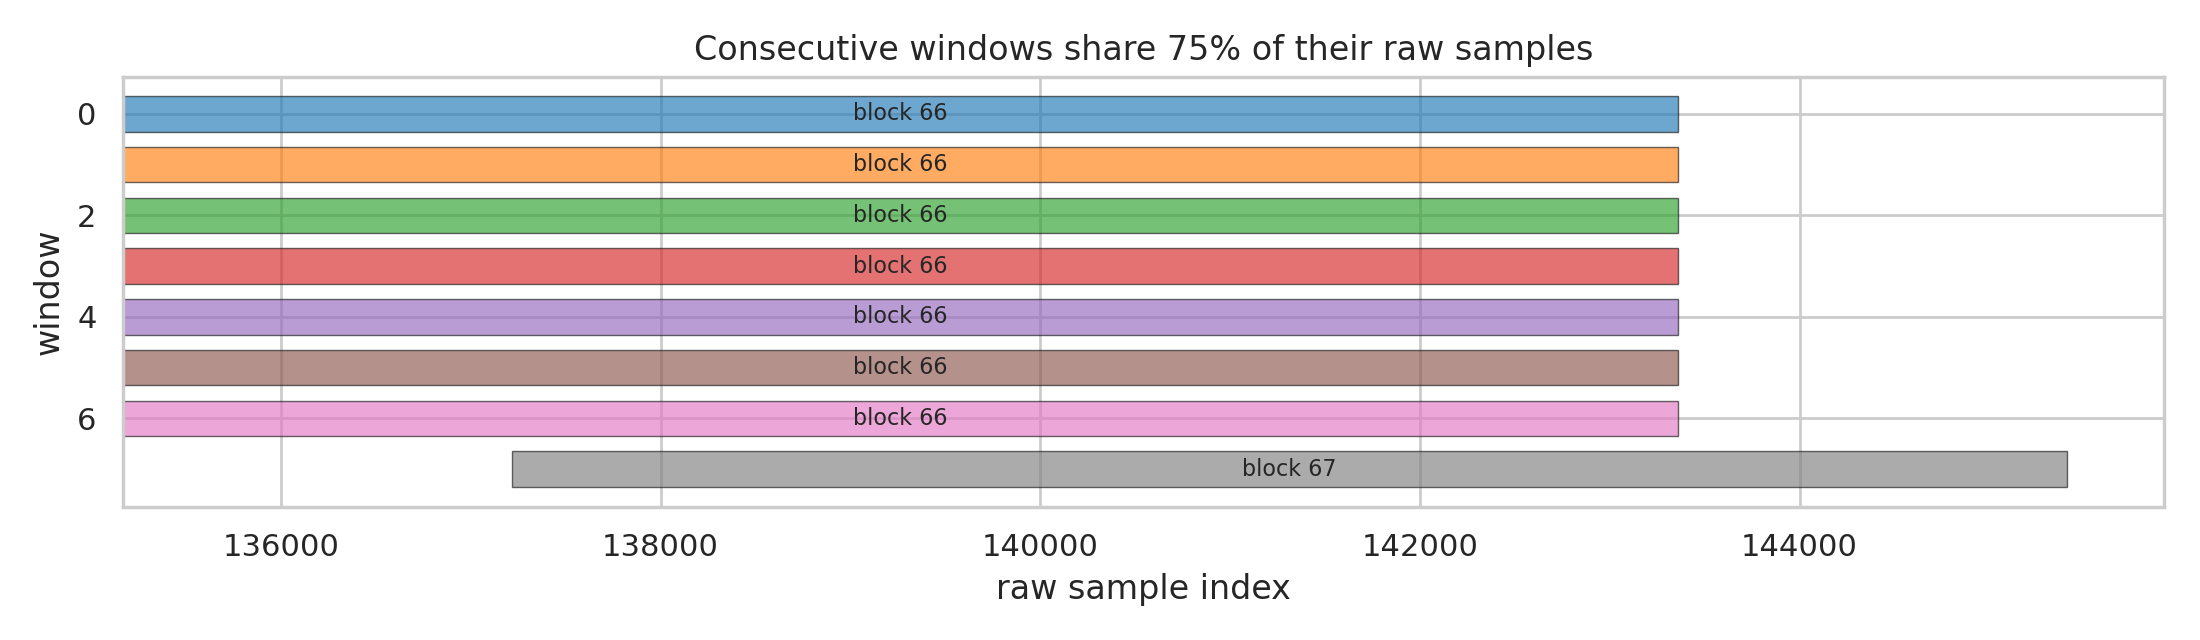
\includegraphics[width=0.9\textwidth,keepaspectratio]{Figures/fig14_window_overlap.png}
\caption{Consecutive analysis windows in the Tomasov dataset share $6{,}144$ of their $8{,}192$ raw samples. Under a random split these overlapping windows are distributed across training, validation, and test.}
\label{fig:window_overlap}
\end{figure}

\paragraph[Step 2: The Recording Inventory]{Step 2: The Recording Inventory.}
The second step tabulated the Tomasov windows by class and by recording (Table~\ref{tab:dataset}). The $439{,}754$ windows come from only 16 recordings, and five of the nine classes, \emph{openclose} among them, are each drawn from a single recording. For these classes the event label and the recording identity are the same variable, so any property of the recording, such as its noise floor, coupling, or local fibre geometry, predicts the label perfectly. This observation explained why the first-cycle result for \emph{openclose} deserved suspicion. All $6{,}792$ of its windows come from one recording spanning only 128 annotated blocks, about 13\,s of signal, so under a random partition almost every test window had near-duplicates from the same few seconds of the same recording in the training set.

\paragraph[Step 3: The Session Structure of the Cao Release]{Step 3: The Session Structure of the Cao Release.}
The Cao release seems at first to avoid the problem, because it ships as pre-segmented, non-overlapping records already divided into fixed training and test folders. Its filenames, however, follow the pattern \texttt{date\_operator\_event\_session\_data\_N}, which shows that many records were cut from each continuous recording session. Every record from one session shares the fibre state, coupling, background-noise realisation, and operator of that session, so the session rather than the record is the unit of independence, just as the subject rather than the record is the unit of independence in clinical sensor data~\cite{saeb2017usecase}. Whether the released partition respects that unit cannot be read from the folder structure; it had to be measured.

\paragraph[Step 4: Quantifying the Contamination]{Step 4: Quantifying the Contamination.}
Two audits turned these observations into measurements, and both operate on the manifests without reading any signal data. For Tomasov, which has no released partition, the audit applies the first-cycle protocol, a stratified random $80/10/10$ partition, to all $439{,}754$ annotated windows under the study's fixed seed. For every recording it marks each raw-sample block read by any training window and counts the test windows whose read interval intersects that training footprint. For Cao, the audit counts, for each of the 441 sessions recovered from the filenames, the records it contributes to each released folder, and flags a session as contaminated when both counts are non-zero. The Tomasov audit finds that all $43{,}976$ test windows (100\%) share raw samples with at least one training window. The Cao audit finds 423 of 441 sessions (95.9\%) contaminated, which places $3{,}083$ of the $3{,}084$ records in the released test folder in a session that also supplies training records. \refs{sec:resLeakage} reports both audits in full.

\paragraph[Step 5: Linking Contamination to Performance]{Step 5: Linking Contamination to Performance.}
Contamination shows that a protocol can be exploited, but not that reported accuracy was actually inflated. The final step tested that link directly through controlled comparisons in which a model is trained twice with every factor held fixed except the partition: once under the leakage-controlled partition developed below, and once under a random partition of the same windows. Any difference between the two arms is attributable to the protocol alone. These protocol-attribution experiments, defined in \refss{sec:chap3ConfoundDesign}, are applied to the reconstructed Tomasov CNN, to every feature configuration of the pipeline, and to five recent architectures. Chapter~\ref{chap:ResultsAndDiscussion} reports their results, together with the change in per-class performance once the leak is removed.

\paragraph[Leakage Pathways and Their Controls]{Leakage Pathways and Their Controls.}
The investigation established two leakage pathways that originate in the data. Three further pathways do not depend on the data at all: they arise in the modelling pipeline whenever a fitted component, whether a feature selector, a resampler, or a scaler, is exposed to rows that are later used for evaluation (\refss{sec:chap2LeakPipeline}). The controls applied to all five follow the recommendations summarised in Table~\ref{tab:leakage_controls}, and Table~\ref{tab:leak_pathways} lists each pathway with its control. The partitioning scheme of \refss{sec:chap3Partitioning} closes the two data pathways, and confining every fitted component to training rows (\refss{sec:chap3ModelReady}) closes the three pipeline pathways. Each control is enforced by the structure of the code or by an assertion that halts execution, not by convention.

\begin{table}[!htbp]
	\centering
	\caption{Leakage pathways addressed in this study and the control applied to each.}
	\label{tab:leak_pathways}
	\small
	\setlength{\tabcolsep}{4pt}
	\begin{tabularx}{\textwidth}{@{}>{\raggedright\arraybackslash}p{2.2cm} >{\raggedright\arraybackslash}X >{\raggedright\arraybackslash}X >{\raggedright\arraybackslash}p{1.9cm}@{}}
		\toprule
		\textbf{Pathway} & \textbf{Source} & \textbf{Control} & \textbf{Section}\\
		\midrule
		Sample level    & Overlapping Tomasov windows share raw samples in time and across adjacent loci & Blocked segments with guard bands; raw-sample disjointness asserted & \ref{sec:chap3Partitioning}\\
		Recording level & Windows from one session or recording share acquisition conditions & Whole-group assignment (Tomasov: recording segment; Cao: session); group disjointness asserted & \ref{sec:chap3Partitioning}\\
		Selection level & Feature selectors fitted on rows later used for evaluation & Selectors fitted on training rows only and refitted inside every cross-validation fold & \ref{sec:chap3FeatureSelection}\\
		Resampling level & Synthetic samples interpolated across partition boundaries & Resamplers fitted inside the training pipeline and bypassed at prediction & \ref{sec:chap3Balancing}\\
		Scaling level   & Scaling statistics computed on evaluation rows & Scaler fitted inside the training pipeline & \ref{sec:chap3ModelReady}\\
		\bottomrule
	\end{tabularx}
\end{table}

\subsubsection{Group-Aware Partitioning}
\label{sec:chap3Partitioning}
\autoBookmark{subsubsec}{Group-Aware Partitioning}
The partitioning scheme replaces both released protocols. It follows four rules, in the spirit of the blocked cross-validation that Roberts et al.\ recommend for data with temporal, spatial, or hierarchical structure~\cite{roberts2017crossvalidation}, of the subject-wise partitioning required when several samples come from one source~\cite{saeb2017usecase}, and of h-block and hv-block cross-validation, which remove a band of observations between training and test data~\cite{burman1994hblock,racine2000hvblock}. First, a partition boundary may fall only between whole groups of dependent samples, never inside one. Second, each dataset targets an approximate $80/10/10$ division into training, validation, and test sets. Third, every class must be present in every split, since per-class metrics are otherwise undefined. Fourth, the partition is computed once from the manifest, before any feature is extracted, and frozen to disk; every later experiment joins against the stored assignment and none re-derives it. Because the two datasets have different dependence structures, the first rule is implemented differently for each.

\paragraph[Tomasov: Blocked Partitioning by Equal-Mass Segments]{Tomasov: Blocked Partitioning by Equal-Mass Segments.}
Two simpler alternatives were ruled out first. Leave-one-recording-out partitioning cannot cover the full taxonomy, because each single-recording class would vanish from training whenever its recording is held out. Stratified group $k$-fold over fixed-duration zones balances the number of groups per fold rather than the number of windows, and a zone in this dataset holds anywhere from 30 to $8{,}000$ windows depending on how many loci the event touches; the resulting $92/5/2$ partition left \emph{openclose} with no test samples at all. The adopted scheme therefore partitions each recording internally along its timeline (Algorithm~\ref{alg:blocked}). The windows of a recording are ordered by block index and divided at the deciles of that ordering into ten contiguous segments of approximately equal \emph{window mass}, and each segment boundary is moved to a block boundary so that no block is shared between segments. A random offset $o_r \in \{0, \dots, 9\}$, drawn for each recording from a generator seeded with the study seed, selects segment $o_r$ for validation and segment $(o_r + 1) \bmod 10$ for test, and the remaining eight segments form the training set. Rotating the offset prevents the held-out data from always lying at the start or end of a recording, where acquisition drift would otherwise be confounded with the split. Each recording--segment pair is one split group, giving 154 groups in total.

\begin{algorithm}[!htbp]
	\caption{Blocked partitioning of one Tomasov recording with guard bands.}
	\label{alg:blocked}
	\DontPrintSemicolon
	\KwIn{Manifest rows of recording $r$ with block indices $b_i$; number of segments $S = 10$; window span $B = L/H = 4$ blocks; guard width $G = 4$ blocks; seeded generator $\rho$}
	\KwOut{Split tag and retention flag for every row of $r$}
	Sort the rows by $b_i$ and compute the rank quantile $q_i \in [0, 1)$ of each row\;
	$s_i \leftarrow \lfloor S\, q_i \rfloor$, then $s_i \leftarrow \min\{s_j : b_j = b_i\}$ so that no block spans two segments\;
	Draw an offset $o_r$ uniformly from $\{0, \dots, S - 1\}$ using $\rho$\;
	Tag segment $o_r$ as \textit{val}, segment $(o_r + 1) \bmod S$ as \textit{test}, and every other segment as \textit{train}\;
	\ForEach{split $k \in \{\textit{train}, \textit{val}, \textit{test}\}$}{
		$F_k \leftarrow \bigcup_{i \in k} \{b_i, \dots, b_i + B - 1\}$ \tcp*{footprint of $k$}
		$\hat{F}_k \leftarrow \{\, b : |b - b'| \le G \text{ for some } b' \in F_k \,\}$ \tcp*{dilate by $G$}
	}
	\ForEach{row $i$ assigned to split $k$}{
		$\mathrm{keep}_i \leftarrow \bigl[\, \{b_i, \dots, b_i + B - 1\} \cap \bigcup_{k' \neq k} \hat{F}_{k'} = \emptyset \,\bigr]$\;
	}
\end{algorithm}

\paragraph[Guard Bands]{Guard Bands.}
Assigning whole segments makes the split groups disjoint, but not the raw samples, because a training window that begins up to three blocks before a test segment reads blocks inside it. For each recording and split, the footprint of the split is therefore computed as the set of blocks read by any of its windows at any locus, and that footprint is dilated by a guard of $G = L/H = 4$ blocks, one full window length. Any window whose read interval intersects the dilated footprint of a different split is removed. Taking the footprint over all loci makes the guard conservative: after removal, windows in different splits share no time sample at any channel, which also eliminates the spatial near-duplicates identified in Step~1. Guard-band removal deletes $39{,}560$ windows, $9.00\%$ of the annotated set, and shifts the realised division from $79.98/9.96/10.06$ to $84.63/7.61/7.75$. The shift arises because every boundary costs each adjacent split a similar number of windows, which is a much larger fraction of a single validation or test segment than of the eight-segment training block. \reff{fig:split_timeline} shows the resulting assignment along each recording, with the guard bands visible as gaps.

\begin{figure}[!htbp]
\centering
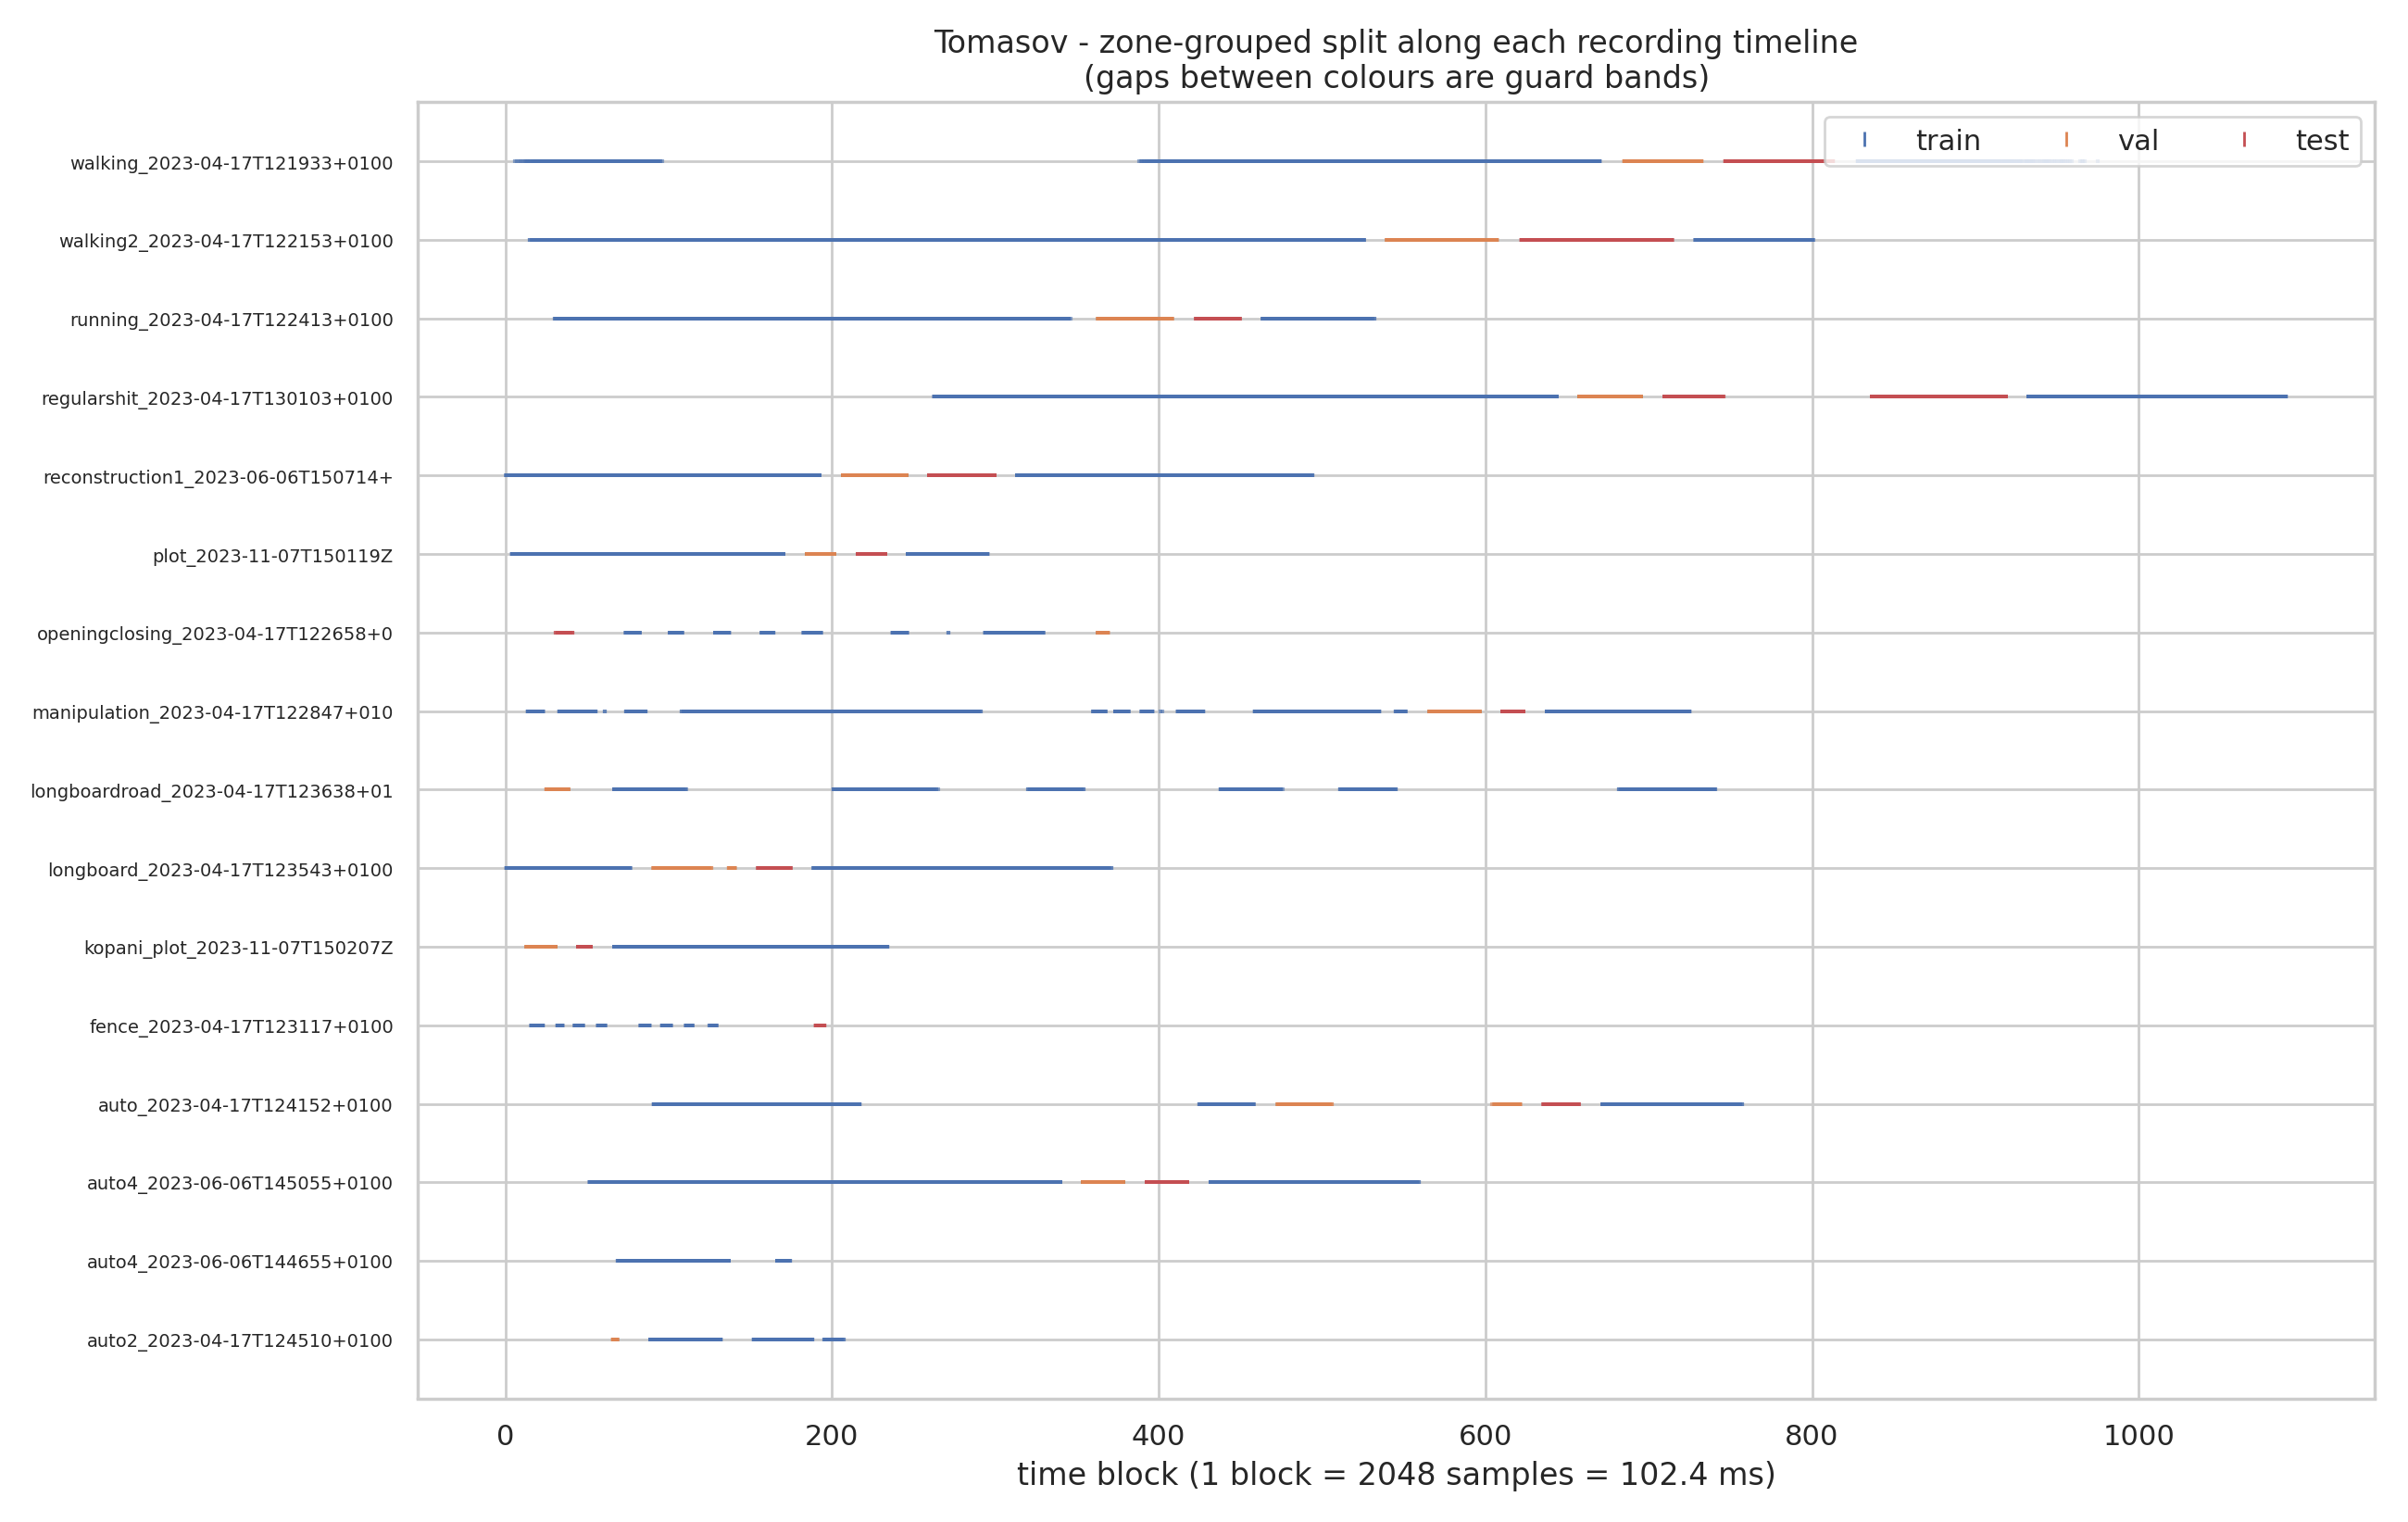
\includegraphics[width=0.95\textwidth,keepaspectratio]{Figures/fig15_split_timeline.png}
\caption{Blocked partitioning of the Tomasov dataset. Each row is one recording and colour denotes split; gaps are guard bands, removed so that no raw sample is shared between splits.}
\label{fig:split_timeline}
\end{figure}

\paragraph[Class Decimation After Partitioning]{Class Decimation After Partitioning.}
Three classes dominate the Tomasov annotations, and \emph{regular} alone accounts for $47.8\%$ of all windows. To stop these classes from dominating training, they are capped at $12{,}350$ (\emph{regular}), $29{,}010$ (\emph{car}), and $27{,}420$ (\emph{construction}) windows, the targets used in the first design cycle, retained for comparability. The first cycle decimated before partitioning; here decimation follows partitioning and guard-band removal, so that the split geometry cannot depend on which windows survive. Within every (class, split) cell the same fraction of windows is drawn at random under the fixed seed, which preserves each class's split proportions. Decimation removes a further $227{,}736$ windows and reduces the imbalance ratio from $30.9{:}1$ in the annotated set to $6.6{:}1$, leaving the $172{,}458$ windows on which features are extracted and every Tomasov result is computed. Because decimation only deletes whole windows, it can shrink but never enlarge the raw-sample footprint of any split, so it cannot reintroduce overlap. Cao is balanced to $1.3{:}1$ as released and is not decimated.

\paragraph[Cao: Session-Grouped Partitioning]{Cao: Session-Grouped Partitioning.}
For Cao the split group is the recording session. Sessions are distributed over ten folds by stratified group $k$-fold with shuffling under the fixed seed, which places each session in exactly one fold while keeping the class distribution of each fold as close to the overall distribution as indivisible sessions allow. Eight folds are merged into the training set, and the remaining two become the validation and test sets. Each record is a separate, non-overlapping segment, so no two records share raw samples and no guard band is needed. Sessions vary in size, so moving whole sessions cannot meet the target exactly; the realised division is $78.84/9.47/11.69$, with 351, 46, and 44 sessions in the three splits. The same operator or acquisition date may still appear in more than one split. This is deliberate, since forbidding it would leave several classes without training data, and the stricter question of generalisation to an unseen acquisition date is answered separately by the leave-one-date-out evaluation of \refss{sec:chap3ConfoundDesign}.

\paragraph[Verification]{Verification.}
Four properties are asserted in code before any model is trained, and the pipeline halts if any of them fails: (i) no split group appears in more than one split; (ii) no sample identifier is duplicated; (iii) for Tomasov, the sets of raw-sample blocks read by the three splits are pairwise disjoint within every recording; and (iv) every class is present in every split. The fourth property is checked rather than assumed. Aligning segments with blocks can merge neighbouring segments, and the guard bands can empty a short segment entirely, so an individual recording may contribute to fewer than three splits. In the final partition, two of the four \emph{car} recordings and one of the two \emph{longboard} recordings contribute no test windows, yet every class remains represented in every split. The full verification is run after guard-band removal and repeated on the decimated manifest, so the guarantees hold on the exact windows used for training and evaluation rather than on a superset of them. \refss{sec:chap3RealisedPartitions} reports the realised sizes at each stage.

\subsection{Signal Preprocessing}
\label{sec:chap3Preprocessing}
\autoBookmark{subsec}{Signal Preprocessing}
Preprocessing turns raw interrogator output into a quantity that a feature extractor can describe meaningfully. It matters more in DAS than in many sensing modalities, because the raw measurement carries several contaminants on different timescales, and any left in place would be absorbed into the descriptors as though it were information about the event. This subsection states what each operation removes, why the operations are ordered as they are, and what the chain costs. \reff{fig:example_window} shows one annotated Tomasov window before and after conditioning.

\begin{figure}[!htbp]
\centering
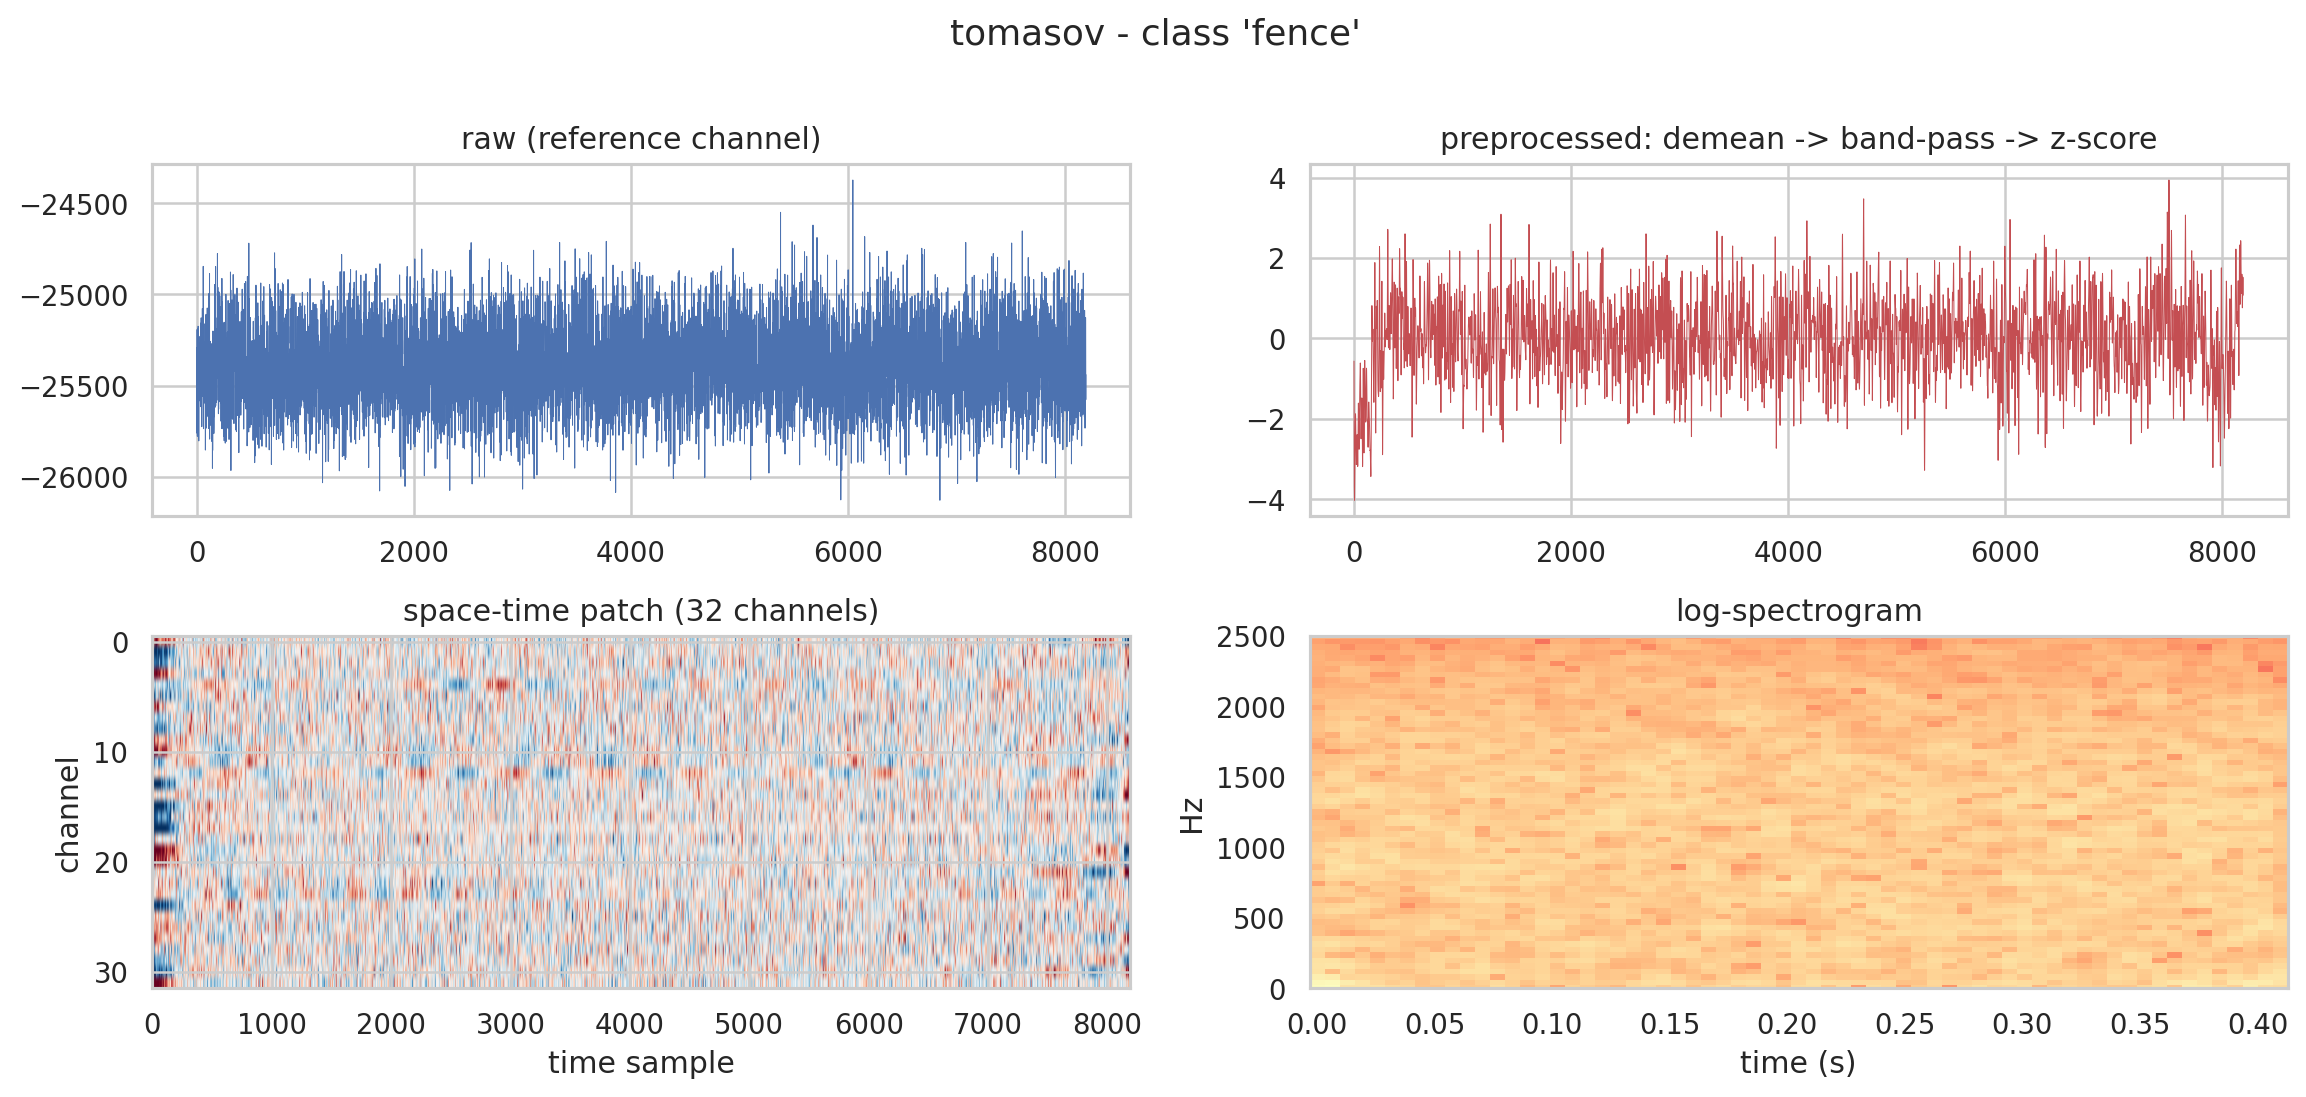
\includegraphics[width=0.95\textwidth,keepaspectratio]{Figures/fig28_example_window_fence.png}
\caption{One annotated \emph{fence} window from the Tomasov dataset: raw reference channel (top left), the same channel after demeaning, band-pass filtering, and z-scoring (top right), the 32-channel space--time patch used by the spatial extractor (bottom left), and the log-spectrogram used by the time--frequency extractor (bottom right).}
\label{fig:example_window}
\end{figure}

\subsubsection{The Raw Signal in DAS}
\label{sec:chap3RawSignal}
\autoBookmark{subsubsec}{The Raw Signal in DAS}
A single DAS channel records the optical phase, or the backscattered intensity, at one point along the fibre, and the recorded quantity superimposes four components on the vibration of interest. They operate on different timescales and call for different treatment, which is why the conditioning chain has three stages rather than one.

\begin{enumerate}[label=(\roman*), leftmargin=*, itemsep=3pt]
	\item \textbf{A large, slowly varying offset and drift.} Thermal expansion, laser wavelength drift, and slow strain accumulation produce a low-frequency component that often exceeds the event in magnitude. Left in place, it dominates every amplitude statistic and every low-frequency spectral bin.
	\item \textbf{Broadband instrument and shot noise.} Detector and digitisation noise extend across the full band, contributing energy unrelated to any event and varying with interrogator settings.
	\item \textbf{Coherent fading.} Backscatter from a given locus can interfere destructively, so that the channel intermittently loses sensitivity. This is a channel-specific, time-varying gain effect rather than additive noise, and it is one reason the spatial descriptors must be read with care.
	\item \textbf{Acquisition-specific gain.} The absolute amplitude scale depends on interrogator configuration, fibre coupling, and burial conditions, all fixed within a recording and different between recordings.
\end{enumerate}

Demeaning and band-pass filtering address components (i) and (ii), and amplitude normalisation addresses component (iv), for reasons given in \refss{sec:chap3Normalisation}. Component (iii) is a time-varying, channel-specific gain that cannot be estimated from a single window, so it is carried as a known limitation in the interpretation of the spatial domain rather than corrected. The subsections below define the unit of analysis and then take the three operations in the order in which they are applied.

\subsubsection{Windowing}
\label{sec:chap3Windowing}
\autoBookmark{subsubsec}{Windowing}
Both datasets are reduced to a common unit of analysis before conditioning. For Tomasov, the continuous stream is divided into windows of $T = 8{,}192$ samples advanced by $H = 2{,}048$ samples, matching the geometry on which the released annotation mask is defined: the mask marks (time-block, locus) cells where a block is $H$ raw samples, so a window beginning at block $b$ reads blocks $b$ to $b + L/H - 1$. This correspondence is what makes the guard-band computation of \refss{sec:chap3Partitioning} exact.

For Cao, records are already segmented at $10{,}000$ samples, and each record yields exactly one window. A centre crop of $8{,}192$ samples is taken, discarding 904 samples at each end, so that every window in the study has the same length and a single extractor serves both datasets. Because the authors clipped each record with the disturbance positioned mostly at its centre, the crop keeps the event and removes only the record margins. One window per record also means that Cao windows never overlap, which is why the sample-level pathway of Table~\ref{tab:leak_pathways} applies to Tomasov alone.

Two objects are produced per window and carried forward: a one-dimensional signal $x \in \mathbb{R}^{T}$, used by the time, frequency, and time--frequency extractors, and a two-dimensional space--time patch $X \in \mathbb{R}^{C \times T}$, used by the spatial extractor. For Tomasov, $C = 32$ loci centred on the annotated channel, and the one-dimensional signal is the centre channel of that patch. For Cao, $C = 12$ (all loci of the record), and the one-dimensional signal is the highest-energy channel, which corresponds to the disturbance location.

\subsubsection{Direct-Current Removal}
\label{sec:chap3DCRemoval}
\autoBookmark{subsubsec}{Direct-Current Removal}
The first operation subtracts the window mean:
\begin{equation}
	x^{(1)} = x - \mu_x, \qquad \mu_x = \frac{1}{T}\sum_{t=1}^{T} x_t .
	\label{eq:dcremoval}
\end{equation}
Demeaning precedes filtering for a practical reason. The band-pass filter is applied by forward--backward recursion, and a large constant offset at the boundaries of a finite window produces a transient that contaminates the first and last several hundred samples. Removing the offset first reduces that transient by roughly the size of the offset.

\subsubsection{Band-Pass Filtering}
\label{sec:chap3Filtering}
\autoBookmark{subsubsec}{Band-Pass Filtering}
A fourth-order Butterworth band-pass filter with cut-offs $f_{\mathrm{low}} = 20$\,Hz and $f_{\mathrm{high}} = 2000$\,Hz is applied next. The Butterworth response is chosen for its maximally flat passband, which avoids imposing ripple on the spectral shape that the frequency-domain descriptors are meant to measure. Fourth order gives a $-24$\,dB/octave roll-off, enough to suppress drift while keeping the transition band narrow enough not to attenuate the low end of the event band.

The band limits follow the physics of the events. The 20\,Hz lower edge sits above thermal and slow-strain drift and below the fundamental of footstep and vehicle excitation. The 2000\,Hz upper edge keeps the transient content of impacts and digging while discarding a region of the spectrum that, in these recordings, carries mainly instrument noise. The upper edge is clipped to $0.99$ times the Nyquist frequency of whichever dataset is being processed, so one specification serves both the 20\,kHz Tomasov stream and the slower Cao acquisition.

Filtering uses a second-order-sections implementation applied forward and backward. The cascaded biquad form stays numerically stable at these cut-off ratios, where a direct-form fourth-order filter would be poorly conditioned, and forward--backward application yields zero phase distortion. That matters because several descriptors (burst structure, envelope moments, spatial-centroid trajectory) depend on the temporal position of signal features. The cost is a doubling of the effective filter order, which is accounted for in the stated roll-off. Writing $\mathcal{H}_{\mathrm{BP}}(\cdot)$ for this operation,
\begin{equation}
	x^{(2)} = \mathcal{H}_{\mathrm{BP}}\!\left(x^{(1)}\right).
	\label{eq:bandpass}
\end{equation}

\subsubsection{Amplitude Normalisation}
\label{sec:chap3Normalisation}
\autoBookmark{subsubsec}{Amplitude Normalisation}
The final operation standardises the filtered window to zero mean and unit variance:
\begin{equation}
	\tilde{x} = \frac{x^{(2)} - \mu_{\mathcal{H}}}{\sigma_{\mathcal{H}}},
	\label{eq:zscore}
\end{equation}
where $\mu_{\mathcal{H}}$ and $\sigma_{\mathcal{H}}$ are the mean and standard deviation of the filtered signal. The implementation evaluated in this thesis adds $\epsilon = 10^{-12}$ to the denominator as a guard against silent channels, a choice whose side effect is examined in \refss{sec:chap5LimResidue}. Combining Equations~\eqref{eq:dcremoval}--\eqref{eq:zscore} gives the complete chain:
\begin{equation}
	\tilde{x} = \frac{\mathcal{H}_{\mathrm{BP}}(x - \mu_x) - \mu_{\mathcal{H}}}{\sigma_{\mathcal{H}}}.
	\label{eq:preprocess}
\end{equation}

This step needs justification, because discarding absolute amplitude discards real information: a passing vehicle does excite the fibre more strongly than a footstep. The decision rests on the group structure of \refss{sec:chap3Dataset}. Absolute amplitude in DAS is set by interrogator gain and fibre coupling, constant within a recording and different between recordings. With five of nine Tomasov classes drawn from a single recording each, an amplitude-preserving representation would hand the classifier a near-perfect recording fingerprint, and with it a shortcut to the label that no deployment could reproduce. Per-window normalisation is designed to remove that shortcut. It is therefore a leakage control first and a numerical convenience second, and its measured cost is accepted.

Two consequences follow. A few amplitude descriptors become constant by construction, since after normalisation the window mean is zero and the standard deviation one; the variance filter in the selection ensemble (\refss{sec:chap3Phase3}) removes them, which is one of the roles that filter serves. A ratio descriptor defined as the coefficient of variation would divide by a mean that is now zero, so its slot in the time-domain vector is taken by the scale-invariant ratio of root-mean-square to median absolute deviation, which measures the same notion of peakedness without the singularity.

\subsubsection{Properties of the Chain}
\label{sec:chap3PreprocProperties}
\autoBookmark{subsubsec}{Properties of the Chain}
Three properties of the chain matter for the validity of the evaluation. It is \textbf{stateless}: every parameter used to transform a window is computed from that window alone, so preprocessing cannot transfer information between samples or splits and may safely be applied before partitioning, whereas classifier feature scaling may not and is placed inside the training pipeline. It is \textbf{identical across datasets}: the same three operations with the same parameters, apart from Nyquist clipping, are applied to both acquisitions, so any difference in outcome is attributable to the data. And it is \textbf{applied per channel} for the two-dimensional patch: Equations~\eqref{eq:dcremoval}--\eqref{eq:zscore} are applied independently to each of the $C$ channels, which removes the per-channel gain differences caused by coupling variation and fading. It also gives every channel the same total energy, a consequence taken up in \refss{sec:chap3SpatialFeatures}.

\subsubsection{Computational Cost}
\label{sec:chap3PreprocCost}
\autoBookmark{subsubsec}{Computational Cost}
Preprocessing is cheap relative to feature extraction. The dominant term is the forward--backward filter, $\mathcal{O}(T)$ per channel with a small constant, applied $C$ times for the patch. On the target embedded platform conditioning takes a negligible fraction of the per-window budget reported in \refss{sec:chap3Efficiency}, which the time--frequency descriptors dominate by two orders of magnitude. The preprocessing parameters were therefore chosen on signal-quality grounds without a runtime constraint.

\subsection{Multi-Domain Feature Extraction and Fusion}
\label{sec:chap3Phase2}
\autoBookmark{subsec}{Multi-Domain Feature Extraction and Fusion}
Feature extraction builds a compact, discriminative description of each preprocessed window. Instead of relying on one representation, handcrafted descriptors are drawn from four complementary domains (\reff{fig:feature_extraction}). Time-domain descriptors capture amplitude and morphology, frequency-domain descriptors capture spectral structure, time--frequency descriptors capture non-stationary behaviour, and spatial and spatio-temporal descriptors exploit how energy localises and propagates across channels. Each family is defined below, and Table~\ref{tab:dimensionality} collects the counts.

\WarningFilter[frameworkfloat]{latex}{Float too large for page}
\ActivateWarningFilters[frameworkfloat]
\clearpage
\begin{landscape}
\makeatletter
\def\LS@rot{%
    \setbox\@outputbox\vbox{\hbox{\rotatebox[origin=c]{-90}{\box\@outputbox}}}%
}
\PLS@Rotate{270}
\makeatother
\begin{figure}[p]
    \centering
    \vspace*{-2.5cm}
    \makebox[\linewidth][c]{%
        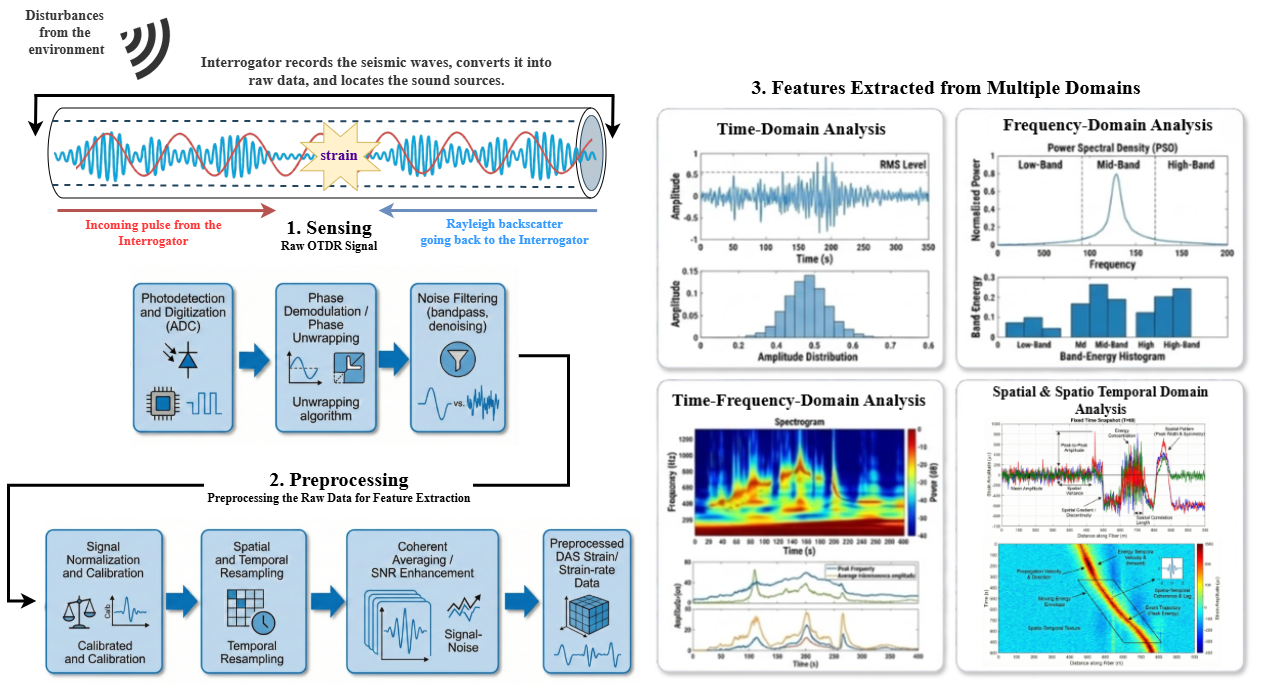
\includegraphics[
            width=0.88\paperheight,
            height=0.84\paperwidth,
            keepaspectratio
        ]{Figures/fig05_FE_pipeline.png}%
    }
    \caption{Feature extraction pipeline for DAS, spanning the time, frequency, time--frequency, and spatial/spatio-temporal domains.}
    \label{fig:feature_extraction}
\end{figure}
\end{landscape}
\DeactivateWarningFilters[frameworkfloat]
\clearpage

\subsubsection{Time-Domain Features}
\label{sec:chap3TimeFeatures}
\autoBookmark{subsubsec}{Time-Domain Features}
Time-domain features summarise amplitude, variability, and temporal morphology, and their low cost makes them attractive for real-time pipelines. A total of 112 are computed per window in eight groups: basic statistics, energy and power, temporal activity, slope and derivative measures, nonlinear descriptors, envelope metrics, burst structure, and histogram descriptors (Table~\ref{tab:timefeatures}). Let $x = [x_1, \ldots, x_N]$ denote a preprocessed window.

The standard moments, mean ($\mu$), variance ($\sigma^2$), skewness ($\gamma_1$), and kurtosis ($\gamma_2$), are
\begin{equation}
	\mu = \frac{1}{N}\sum_{i=1}^{N} x_i, \qquad \sigma^2 = \frac{1}{N}\sum_{i=1}^{N}(x_i - \mu)^2,
	\label{eq:meanvar}
\end{equation}
\begin{equation}
	\gamma_1 = \frac{\frac{1}{N}\sum_{i=1}^{N}(x_i - \mu)^3}{(\sigma^2)^{3/2}}, \qquad
	\gamma_2 = \frac{\frac{1}{N}\sum_{i=1}^{N}(x_i - \mu)^4}{(\sigma^2)^2}.
	\label{eq:skewkurt}
\end{equation}
Further statistics include percentiles, the interquartile range, the median absolute deviation, and the zero fraction. Energy features quantify signal strength through the root-mean-square value and the signal energy,
\begin{equation}
	\mathrm{RMS} = \sqrt{\frac{1}{N}\sum_{i=1}^{N} x_i^2}, \qquad E_{\mathrm{signal}} = \sum_{i=1}^{N} x_i^2,
	\label{eq:rmsenergy}
\end{equation}
and shape factors such as the crest factor detect transient peaks:
\begin{equation}
	\mathrm{CF} = \frac{\max(|x|)}{\mathrm{RMS}}.
	\label{eq:crest}
\end{equation}
The window is also divided into $K = 10$ segments to compute segment energies together with their entropy, centroid, spread, and Gini coefficient. Temporal activity is described by the zero-crossing rate, peak and valley counts, activity factors, and autocorrelation statistics, where
\begin{equation}
	\mathrm{ZCR} = \frac{1}{2(N-1)}\sum_{i=1}^{N-1} \bigl|\operatorname{sgn}(x_{i+1}) - \operatorname{sgn}(x_i)\bigr| \times f_s .
	\label{eq:zcr}
\end{equation}
Slope features include the mean and variance of the first difference ($\Delta x_i = x_{i+1} - x_i$) and of the second difference, together with slope-sign changes and waveform length. The Hjorth parameters, activity ($A$), mobility ($M$), and complexity ($C$), capture signal dynamics:
\begin{equation}
	A = \operatorname{var}(x), \qquad
	M = \sqrt{\frac{\operatorname{var}(\Delta x)}{\operatorname{var}(x)}}, \qquad
	C = \frac{\sqrt{\operatorname{var}(\Delta^2 x)/\operatorname{var}(\Delta x)}}{M}.
	\label{eq:hjorth}
\end{equation}
The Katz fractal dimension, from the curve length $L$ and maximum displacement $d$, is
\begin{equation}
	D_K = \frac{\log_{10}(N)}{\log_{10}(N) + \log_{10}(d/L)},
	\label{eq:katz}
\end{equation}
and the Higuchi fractal dimension and Teager--Kaiser energy complete the nonlinear group. Hilbert-envelope statistics describe modulation, and thresholding the envelope yields burst count, rate, duration, gap, and occupancy.

\begin{table}[!htb]
	\centering
	\caption{Summary of time-domain feature groups.}
	\label{tab:timefeatures}
	\small
	\setlength{\tabcolsep}{4pt}
	\renewcommand{\arraystretch}{0.95}
	\begin{tabularx}{\textwidth}{@{}>{\raggedright\arraybackslash}p{3.1cm} c >{\raggedright\arraybackslash}X@{}}
		\toprule
		\textbf{Feature Group} & \textbf{Count} & \textbf{Description}\\
		\midrule
		Basic statistical   & 26       & Central tendency, dispersion, percentiles, distribution shape, zero fraction.\\
		Energy \& power     & $13 + K$ & RMS, energy, shape factors, and $K = 10$ segment energies with their entropy, centroid, spread, and Gini coefficient.\\
		Temporal patterns   & 19       & Zero crossings, peak and valley statistics, activity factors, autocorrelation.\\
		Slope \& derivative & 7        & First and second differences, slope-sign changes, waveform length.\\
		Nonlinear descriptors & 7      & Hjorth parameters, Katz and Higuchi fractal dimensions, Teager--Kaiser energy.\\
		Envelope-based      & 6        & Moments, entropy, and crest of the Hilbert envelope.\\
		Burst structure     & 6        & Burst count, rate, duration, gap, and occupancy.\\
		Histogram-based     & 18       & 16-bin amplitude histogram with entropy and contrast.\\
		\midrule
		\textbf{Total}      & \textbf{112} & \\
		\bottomrule
	\end{tabularx}
\end{table}

\subsubsection{Frequency-Domain Features}
\label{sec:chap3FreqFeatures}
\autoBookmark{subsubsec}{Frequency-Domain Features}
Frequency-domain features summarise how vibration energy is distributed across frequencies and separate events with distinct spectral signatures. Each window is transformed with the real-valued FFT and 90 descriptors are extracted (Table~\ref{tab:freqfeatures}). The spectrum of a window $x[n]$ is
\begin{equation}
	X[k] = \sum_{n=0}^{N-1} x[n]\, e^{-j 2\pi k n / N}, \qquad k = 0, 1, \ldots, \tfrac{N}{2},
	\label{eq:fft}
\end{equation}
from which the magnitude spectrum $M[k] = |X[k]|$ and the power spectrum $P[k] = |X[k]|^2$ follow. The spectral centroid $C$ and spread $S$ are
\begin{equation}
	C = \frac{\sum_{k=0}^{K} f_k \, M[k]}{\sum_{k=0}^{K} M[k]}, \qquad
	S = \sqrt{\frac{\sum_{k=0}^{K} (f_k - C)^2 \, M[k]}{\sum_{k=0}^{K} M[k]}},
	\label{eq:centroid}
\end{equation}
where $f_k$ is the frequency at bin $k$. The Shannon spectral entropy of the normalised power spectrum $p_k = P[k] / \sum P[k]$ is
\begin{equation}
	H = -\sum_{k=0}^{K} p_k \log_2 (p_k + \epsilon),
	\label{eq:entropy}
\end{equation}
with $\epsilon$ a small constant that prevents a logarithmic singularity. Band powers are computed in absolute and relative form over seven bands: $[0,50]$, $[50,100]$, $[100,200]$, $[200,400]$, $[400,800]$, $[800,1600]$, and $[1600, f_s/2]$\,Hz.

\begin{table}[!htbp]
	\centering
	\caption{Summary of frequency-domain feature groups.}
	\label{tab:freqfeatures}
	\small
	\begin{tabularx}{\textwidth}{@{}>{\raggedright\arraybackslash}p{3.4cm} c >{\raggedright\arraybackslash}X@{}}
		\toprule
		\textbf{Feature Group} & \textbf{Count} & \textbf{Description}\\
		\midrule
		Basic spectral statistics & 8  & Mean, std, min, max, and range of magnitude and power.\\
		Spectral shape            & 8  & Centroid, spread, roll-off, flatness, skewness, kurtosis, slope.\\
		Peak-related              & 6  & Dominant and secondary peak frequency and amplitude; peak count and ratio.\\
		Band powers               & 14 & Absolute and relative power in seven bands.\\
		DAS band ratios           & 7  & Low/mid/high energy ratios, fractions, and high-tail ratio.\\
		Spectral entropy          & 3  & Shannon entropy, R\'enyi entropy, spectral decrease.\\
		PSD statistics            & 3  & Max, min, and range of power spectral density.\\
		Histogram features        & 33 & 32-bin magnitude histogram and its entropy.\\
		Cepstral coefficients     & 8  & First eight real cepstral coefficients.\\
		\midrule
		\textbf{Total}            & \textbf{90} & \\
		\bottomrule
	\end{tabularx}
\end{table}

\subsubsection{Time--Frequency-Domain Features}
\label{sec:chap3TFFeatures}
\autoBookmark{subsubsec}{Time--Frequency-Domain Features}
DAS event signatures are often non-stationary, so time--frequency representations are used to model temporal evolution and spectral content jointly. A hybrid set of 739 features combines STFT statistics, wavelet decompositions, texture and geometry descriptors of a quantised log-spectrogram, and DAS-specific indices (Table~\ref{tab:tffeatures}). The magnitude spectrogram $S(m,k)$ is computed with a Hann window, $N_{\mathrm{FFT}} = 512$, and a hop of 128 samples,
\begin{equation}
	S(m,k) = \left| \sum_{n=0}^{N_{\mathrm{FFT}}-1} x[n]\, w[n - mH]\, e^{-j 2\pi k n / N_{\mathrm{FFT}}} \right|,
	\label{eq:stft}
\end{equation}
which gives a $257 \times 61$ spectrogram per window. A coarser $4096/2048$ setting was rejected because it yields only about five frames, too few for the texture descriptors that follow. From $S(m,k)$ are derived global power statistics, temporal-envelope and spectral-marginal descriptors, inter-frame dynamics (flux, divergence, coherence, novelty), a modulation spectrum over 12 critical bands, and the energy in five DAS-relevant bands. Multi-resolution transient behaviour is captured by the discrete wavelet transform (up to level 6) and the wavelet packet transform (full decomposition to level 4, 16 sub-bands), both with the Daubechies-4 wavelet. For each coefficient set $c_i$, statistical moments and the Teager--Kaiser energy
\begin{equation}
	\Psi\bigl[c_i[n]\bigr] = c_i[n]^2 - c_i[n-1]\cdot c_i[n+1]
	\label{eq:tkeo}
\end{equation}
are computed. The log-spectrogram is then quantised to 32 levels, and grey-level co-occurrence statistics, local binary patterns, histogram-of-oriented-gradient features, and morphological descriptors of the binarised time--frequency mask are extracted. Four DAS-specific indices (tonal, transient, cyclostationary, and low--high band ratio) complete the set.

\begin{table}[!htbp]
	\centering
	\caption{Summary of time--frequency feature groups.}
	\label{tab:tffeatures}
	\small
	\begin{tabularx}{\textwidth}{@{}>{\raggedright\arraybackslash}p{3.6cm} >{\raggedright\arraybackslash}X c@{}}
		\toprule
		\textbf{Feature Group} & \textbf{Description} & \textbf{Count}\\
		\midrule
		STFT global power      & Distributional descriptors of spectrogram power (statistics, quantiles, shape moments, entropy). & 16\\
		Temporal envelope ($E_t$) & Statistics of the frequency-integrated power envelope. & 13\\
		Spectral marginal ($E_f$) & Descriptors of the time-integrated spectral distribution. & 21\\
		Spectral dynamics      & Inter-frame flux, divergence, coherence, and novelty. & 8\\
		Modulation spectrum    & Modulation centroid, spread, and entropy across 12 critical bands. & 36\\
		Band power             & Energy in five DAS-relevant bands (0--20, 20--50, 50--150, 150--300, 300--500\,Hz). & 5\\
		DWT features           & Daubechies-4 DWT (levels 0--6): coefficient statistics and TKEO summaries. & 140\\
		WPT features           & Wavelet packet descriptors (level 4, 16 sub-bands): statistics, energy, entropy, ratios. & 357\\
		GLCM texture           & Grey-level co-occurrence statistics over multiple distances and orientations. & 80\\
		LBP histogram          & 32-bin local binary pattern histogram of the quantised spectrogram. & 32\\
		HOG-like features      & 16-bin histogram of oriented gradients of time--frequency edges. & 16\\
		TF geometry            & Morphological descriptors of the binarised time--frequency mask. & 8\\
		TF distribution        & Occupancy and anisotropy measures. & 3\\
		DAS-specific metrics   & Tonal, transient, and cyclostationary indices; low--high band ratio. & 4\\
		\midrule
		\textbf{Total}         & & \textbf{739}\\
		\bottomrule
	\end{tabularx}
\end{table}

\subsubsection{Spatial and Spatio-Temporal Features}
\label{sec:chap3SpatialFeatures}
\autoBookmark{subsubsec}{Spatial and Spatio-Temporal Features}
Unlike a single-channel acoustic sensor, DAS records synchronised measurements across many channels. Each window is modelled as a patch $X \in \mathbb{R}^{C \times T}$, and 61 descriptors quantify how energy localises, spreads, and fragments across channels (Table~\ref{tab:spatialfeatures}). Let $E_c$ denote the energy of channel $c$,
\begin{equation}
	E_c = \sum_{t=1}^{T} |X_{c,t}|^2, \qquad c = 1, \ldots, C,
	\label{eq:channelenergy}
\end{equation}
with total energy $E_{\mathrm{tot}} = \sum_{c} E_c$ and normalised weights $w_c = E_c / (E_{\mathrm{tot}} + \epsilon)$, $\epsilon = 10^{-12}$. The spatial centroid and spread are
\begin{equation}
	\mu_{sp} = \sum_{c=1}^{C} c\, w_c, \qquad
	\sigma_{sp} = \sqrt{\sum_{c=1}^{C} (c - \mu_{sp})^2\, w_c},
	\label{eq:spatialcentroid}
\end{equation}
and the inequality of the channel-energy distribution is the Gini coefficient of the sorted energies $E_{(k)}$:
\begin{equation}
	\mathrm{Gini}(E) = \frac{C + 1 - 2\left(\dfrac{\sum_{k=1}^{C}(C + 1 - k)\, E_{(k)}}{\sum_{k=1}^{C} E_k}\right)}{C}.
	\label{eq:gini}
\end{equation}
Further descriptors capture spatial gradient and roughness (inter-channel differences, edge density, smoothness) and the clustering of active channels. The spatio-temporal group tracks the spatial-centroid trajectory across coarse temporal bins and reports its velocity, directionality, linearity, and variance, together with global patch statistics, the temporal activity profile, gradient and texture measures, and coarse histogram statistics.

\begin{table}[!htb]
	\centering
	\caption{Summary of spatial and spatio-temporal feature groups.}
	\label{tab:spatialfeatures}
	\small
	\setlength{\tabcolsep}{4pt}
	\renewcommand{\arraystretch}{0.95}
	\begin{tabularx}{\textwidth}{@{}>{\raggedright\arraybackslash}p{3.1cm} >{\raggedright\arraybackslash}X c@{}}
		\toprule
		\textbf{Feature Group} & \textbf{Description} & \textbf{Count}\\
		\midrule
		\multicolumn{3}{@{}l}{\textit{Spatial-domain features (from the channel-energy distribution)}}\\[2pt]
		Localisation \& extent     & Centroid, spread, width, argmax, and active-channel counts at thresholds. & 7\\
		Distribution \& shape      & Quantiles, skewness, kurtosis, Gini, entropy, flatness, top-channel fractions. & 10\\
		Gradient \& roughness      & Inter-channel gradient statistics, edge density, smoothness, total variation. & 7\\
		Clustering                 & Cluster count, mean/max/std cluster size, coverage ratio. & 5\\[4pt]
		\multicolumn{3}{@{}l}{\textit{Spatio-temporal features (from the 2D space--time patch)}}\\[2pt]
		Global 2D statistics       & Moments, total energy, and entropy over the patch. & 6\\
		Temporal activity profile  & Active duration, temporal centroid, spread, burstiness, entropy, skew. & 7\\
		Motion \& propagation      & Centroid-trajectory velocity, direction, linearity, variance, range, drift. & 7\\
		Gradient \& texture        & Temporal and channel derivatives, anisotropy, edge densities, gradient correlation. & 8\\
		Coarse texture statistics  & Histogram energy, entropy, contrast, uniformity. & 4\\
		\midrule
		\textbf{Total}             & & \textbf{61}\\
		\bottomrule
	\end{tabularx}
\end{table}

One property of these definitions matters for everything that follows. Because the patch is z-scored per channel (\refss{sec:chap3PreprocProperties}), every channel has the same energy in exact arithmetic, $E_c = T$, and the channel-energy profile is flat. The 29 descriptors in the upper part of Table~\ref{tab:spatialfeatures} are therefore constant by construction, and the spatial information proper lies in the 32 spatio-temporal descriptors, which follow how energy moves between channels within the window. In floating-point execution the 29 are not exactly constant, and \refss{sec:chap5LimResidue} reports what that residue does to the results.

\subsubsection{Multi-Domain Feature Fusion}
\label{sec:chap3Fusion}
\autoBookmark{subsubsec}{Multi-Domain Feature Fusion}
The four domain matrices are fused at feature level by concatenation. This preserves interpretability, because each feature keeps a domain prefix (\texttt{TIME:}, \texttt{FREQ:}, \texttt{TF:}, \texttt{SPAT:}) that remains traceable through selection and attribution. Let $X_{\mathrm{time}} \in \mathbb{R}^{N \times d_t}$, $X_{\mathrm{freq}} \in \mathbb{R}^{N \times d_f}$, $X_{\mathrm{tf}} \in \mathbb{R}^{N \times d_{tf}}$, and $X_{\mathrm{spat}} \in \mathbb{R}^{N \times d_s}$ be the domain matrices for $N$ samples. Once sample counts, identifier order, and label order have been verified identical across the four, the fused matrix is
\begin{equation}
	X_{\mathrm{multi}} = \bigl[\, X_{\mathrm{time}} \oplus X_{\mathrm{freq}} \oplus X_{\mathrm{tf}} \oplus X_{\mathrm{spat}} \,\bigr] \in \mathbb{R}^{N \times D},
	\label{eq:fusion}
\end{equation}
where $\oplus$ denotes concatenation along the feature axis and $D = d_t + d_f + d_{tf} + d_s = 1{,}002$ (Table~\ref{tab:dimensionality}). The fused matrix is then joined to the frozen split manifest by sample identifier, so that the partition is never re-derived downstream. Algorithm~\ref{alg:fusion} gives the procedure.

\begin{table}[!htb]
	\centering
	\caption{Dimensionality of the extracted features per domain.}
	\label{tab:dimensionality}
	\small
	\setlength{\tabcolsep}{4pt}
	\renewcommand{\arraystretch}{0.95}
	\begin{tabular}{@{}lcc@{}}
		\toprule
		\textbf{Signal-Processing Domain} & \textbf{Count} & \textbf{Notation}\\
		\midrule
		Time domain                       & 112  & $d_t$\\
		Frequency domain                  & 90   & $d_f$\\
		Time--frequency domain            & 739  & $d_{tf}$\\
		Spatial \& spatio-temporal domain & 61   & $d_s$\\
		\midrule
		\textbf{Total (multi-domain)}     & \textbf{1{,}002} & $D$\\
		\bottomrule
	\end{tabular}
\end{table}

\begin{algorithm}[!htbp]
	\caption{Multi-domain feature fusion procedure.}
	\label{alg:fusion}
	\DontPrintSemicolon
	\KwIn{Domain feature stores $D_{\mathrm{time}}, D_{\mathrm{freq}}, D_{\mathrm{tf}}, D_{\mathrm{spat}}$; split manifest $\mathcal{M}$}
	\KwOut{Fused matrix $X_{\mathrm{multi}}$, labels $Y$, feature names $F_{\mathrm{multi}}$}
	Load features $X_i$, labels $Y_i$, sample identifiers $s_i$, and names $F_i$ for each domain $i \in \{\mathrm{time, freq, tf, spat}\}$\;
	Prefix feature names: $F_i \leftarrow \{\textsc{domain}_i\!:\!f \mid f \in F_i\}$\;
	Assert $|X_{\mathrm{time}}| = |X_{\mathrm{freq}}| = |X_{\mathrm{tf}}| = |X_{\mathrm{spat}}|$\;
	Assert $s_{\mathrm{time}} \equiv s_i$ and $Y_{\mathrm{time}} \equiv Y_i$ for every domain $i$\;
	$X_{\mathrm{multi}} \leftarrow \mathrm{concat}(X_{\mathrm{time}}, X_{\mathrm{freq}}, X_{\mathrm{tf}}, X_{\mathrm{spat}};\ \mathrm{axis}=1)$\;
	$F_{\mathrm{multi}} \leftarrow F_{\mathrm{time}} + F_{\mathrm{freq}} + F_{\mathrm{tf}} + F_{\mathrm{spat}}$\;
	Join $X_{\mathrm{multi}}$ to $\mathcal{M}$ on sample identifier to attach the split assignment\;
	Save $X_{\mathrm{multi}}$, $Y$, and $F_{\mathrm{multi}}$ to the output directory\;
\end{algorithm}

\paragraph[Single-Pass Extraction]{Single-Pass Extraction.}
Extraction runs in one pass: a window is read once and all four extractors are applied to it, instead of reading and preprocessing the same window once per domain. Work is chunked by recording so that each HDF5 file is opened exactly once, and completed chunks are written as shards so that an interrupted run resumes rather than restarts. Shards are reassembled in a recorded deterministic order, and row counts, column counts, and identifier uniqueness are asserted at assembly.

\subsection{Preparation of Data for Model Training}
\label{sec:chap3ModelReady}
\autoBookmark{subsec}{Preparation of Data for Model Training}
This phase turns the frozen partition manifest and the extracted features into the matrices on which models are fitted and evaluated. Table~\ref{tab:data_objects} traces each dataset from manifest to model input and gives the size of the object produced at every stage. Two decisions govern the path. Extraction is driven by the final partition manifest rather than by the raw files, so features are computed only for windows that survived partitioning, guard-band removal, and decimation, and the $267{,}296$ Tomasov windows removed at those stages are never processed. And no operation that learns from data is applied before the split tags are attached, so the matrices that leave this phase contain raw descriptor values and nothing fitted to any subset of them.

\begin{table}[!htbp]
	\centering
	\caption{Data objects produced between manifest construction and model training, with their sizes for each dataset.}
	\label{tab:data_objects}
	\small
	\setlength{\tabcolsep}{4pt}
	\begin{tabularx}{\textwidth}{@{}>{\raggedright\arraybackslash}p{2.6cm} >{\raggedright\arraybackslash}X >{\raggedleft\arraybackslash}p{2.9cm} >{\raggedleft\arraybackslash}p{2.6cm}@{}}
		\toprule
		\textbf{Stage} & \textbf{Object} & \textbf{Tomasov} & \textbf{Cao}\\
		\midrule
		Manifest       & One row per annotated window & $439{,}754$ & $15{,}418$\\
		Partitioning   & Split manifest after guard bands & $400{,}194$ & $15{,}418$\\
		Decimation     & Final partition manifest & $172{,}458$ & $15{,}418$\\
		Extraction     & Four domain matrices (112, 90, 739, and 61 columns) & $172{,}458$ rows & $15{,}418$ rows\\
		Fusion         & Fused matrix aligned with the manifest & $172{,}458 \times 1{,}002$ & $15{,}418 \times 1{,}002$\\
		Split tagging  & Training rows   & $148{,}229$ & $12{,}155$\\
		               & Validation rows & $12{,}895$  & $1{,}460$\\
		               & Test rows       & $11{,}334$  & $1{,}803$\\
		Selection      & Unanimous consensus columns & 52 & 53\\
		\bottomrule
	\end{tabularx}
\end{table}

Fusion joins the four domain matrices to the partition manifest by sample identifier (Algorithm~\ref{alg:fusion}), and the join is followed by three assertions: every extracted identifier exists in the manifest, no identifier is duplicated, and row $i$ of the fused matrix describes the same window as row $i$ of the aligned manifest. Each row therefore carries, besides its $1{,}002$ features and its label, the split tag, the split group, and the robustness group of its window, so that any later experiment can select rows by these attributes without consulting the raw data. Features are stored in single precision; the Tomasov matrix occupies about 0.69\,GB, comfortably within the unified memory of the embedded platform.

The fused matrix is deliberately left untransformed. Descriptors differ in scale by several orders of magnitude, from ratios near unity to raw spectral energies, but tree ensembles are invariant to monotone rescaling of individual features, and the one scale-sensitive model, logistic regression, receives a scaler inside its training pipeline. Nine features are exactly constant in these matrices, because per-window z-scoring fixes the mean and standard deviation of every window (\refss{sec:chap3Normalisation}); they are kept at this stage and removed later by the variance selector fitted on training data. No row is removed or modified after fusion, so the test set on which results are reported is exactly the test set recorded in the partition manifest.

The split tags then divide the fused matrix into training, validation, and test matrices, and every component that learns from data is fitted on the training matrix alone, in a fixed order. When the consensus subset is used, feature selection is fitted first, on training rows or on class-proportional subsamples drawn from them, and the resulting column mask is applied unchanged to all three matrices. The remaining components form a single imbalanced-learning pipeline in which a scaler, when the model needs one, precedes a resampler, when the balancing strategy uses one, and both precede the classifier. Fitting the pipeline estimates the scaling statistics and synthesises or removes samples using training rows only; at prediction time the fitted scaler is applied and the resampler is bypassed, so validation and test rows are never resampled. Class labels are kept as strings throughout, except for XGBoost, whose labels are integer-encoded by an encoder fitted on the training labels and decoded immediately after prediction, so that every metric is computed in the same label space.

The validation and test matrices play different roles. Every (classifier, balancing strategy) configuration is fitted on the training matrix and scored on both, but only the validation macro-$F_1$ is used to make choices: it selects the balancing strategy retained for each classifier and, across classifiers, the selected configuration. Test scores are reported for the retained configuration of every classifier so that the learners can be compared, but no choice is made on them, and this ordering is enforced in code. Cross-validated estimates are computed on the training matrix alone, with five-fold stratified group $k$-fold over the same split groups as the partition, so that no session or recording segment is divided between folds, and the selection ensemble is refitted inside every fold whenever selection is part of the estimate. Guard bands are not re-applied between folds inside the training set, so windows at the boundary of two adjacent Tomasov training segments placed in different folds may share raw samples. Cross-validated figures are therefore used only for comparisons made within the training data, such as the selection-bias analysis of \refss{sec:chap3ConfoundDesign}, and every headline result is taken from the guarded test partition.

\subsection{Feature Selection, Dimensionality Reduction, and Class Balancing}
\label{sec:chap3Phase3}
\autoBookmark{subsec}{Feature Selection, Dimensionality Reduction, and Class Balancing}

\subsubsection{Ensemble Feature Selection}
\label{sec:chap3FeatureSelection}
\autoBookmark{subsubsec}{Ensemble Feature Selection}
Eight selectors spanning the filter, wrapper, embedded, and explainability families are combined by consensus voting: variance threshold, one-vs-rest Pearson correlation, mutual information, ReliefF~\cite{li2022relieff}, mRMR~\cite{peng2005mrmr}, recursive feature elimination~\cite{guyon2002rfe}, Boruta~\cite{kursa2010boruta}, and SHAP~\cite{lundberg2017shap} (Table~\ref{tab:fsmethods}). Every selector is fitted on training data only, and the expensive methods (mutual information, ReliefF, mRMR, Boruta, and SHAP) use class-proportional subsamples of the training split. Each selector retains its top 50\% of features, and a strict $8/8$ unanimity rule keeps only the features selected by all eight. The selectors embody different criteria (linear and non-linear filters, a redundancy-penalised filter, a tree-based wrapper, a linear-model wrapper, and model attribution), so a unanimous selection has support that does not depend on any one assumption. Pairwise agreement between selectors is measured with the Jaccard index.

\begin{table}[H]
	\centering
	\caption{Feature-selection methods used in the ensemble.}
	\label{tab:fsmethods}
	\scriptsize
	\setlength{\tabcolsep}{3pt}
	\renewcommand{\arraystretch}{0.9}
	\begin{tabularx}{\textwidth}{@{}>{\raggedright\arraybackslash}p{2.45cm} >{\raggedright\arraybackslash}p{2.55cm} >{\raggedright\arraybackslash}X@{}}
		\toprule
		\textbf{Method} & \textbf{Category} & \textbf{Key implementation}\\
		\midrule
		Variance threshold  & Filter, unsupervised & Removes constant or near-constant features, including those made constant by normalisation.\\
		Pearson correlation & Filter, linear & One-vs-rest mean absolute correlation with the label.\\
		Mutual information  & Filter, non-linear & Scaled $k$-NN estimator ($k = 3$) on a $20{,}000$-row training subsample.\\
		ReliefF             & Filter, distance-based & 10 nearest neighbours on a $6{,}000$-row training subsample.\\
		mRMR                & Filter, redundancy-aware & Greedy max-relevance min-redundancy with MI scores, $k = 400$, $20{,}000$ rows.\\
		RFE                 & Wrapper & Logistic regression (LBFGS, 300 iterations, balanced weights), step 0.1.\\
		Boruta              & Wrapper & Balanced random forest, 800 trees, depth 8, 60 iterations, $8{,}000$ rows.\\
		SHAP                & Embedded / explainability & TreeExplainer on a 200-tree random forest of depth 12, $6{,}000$ rows.\\
		\bottomrule
	\end{tabularx}
\end{table}

\paragraph[Fold-Wise Refitting]{Fold-Wise Refitting.}
Whenever a cross-validated estimate is reported, the whole selection ensemble is refitted inside every fold rather than once on the full training split. Fitting selection once and then cross-validating on the same split biases the estimate upward even when the test set is untouched, because each fold has been influenced by the rows it is later asked to predict~\cite{ambroise2002selection,varma2006bias}. \refss{sec:chap3ConfoundDesign} describes the controlled comparison used to measure that bias, and \refss{sec:resSelectionBias} reports it.

\subsubsection{Feature Selection for a Lightweight Model}
\label{sec:chap3LightweightSelection}
\autoBookmark{subsubsec}{Feature Selection for a Lightweight Model}
Feature selection is the stage of the pipeline at which the lightweight requirement of RO1 meets the representation. The fused vector of $1{,}002$ descriptors is chosen for coverage, so that no domain that might separate the events is left out, and every descriptor in it costs something at each later stage: it must be computed for every incoming window, held in memory, searched by the learner at every split during training, and read at every prediction. Unanimous consensus is the most aggressive reduction the design allows, and it is evaluated as a second feature configuration beside the full vector rather than as a replacement for it, so that its effect on the footprint and its cost in accuracy are measured on the same partitions.

Selection can lighten the pipeline in four places, and each is measured rather than assumed. The first is \emph{dimensionality}: the number of descriptors the learner sees, and with it the memory of a stored feature vector at four bytes per value. The second is \emph{training cost}: the time to fit the selected classifier, measured on the same platform and training rows for both configurations. The third is \emph{inference cost and model size}: the per-window prediction time and the stored size of the fitted model, defined as in \refss{sec:chap3Efficiency}. The fourth is \emph{extraction cost}, the largest online cost, which falls only if the extractor computes the retained descriptors alone. The extractor of \refss{sec:chap3Phase2} computes each domain in full, so this saving is not realised in the reported runtimes, and it is treated as future work (\refss{sec:chap5FutureCost}).

Against these savings stand two costs. Selection itself is a one-time offline computation whose time is dominated by the wrapper and attribution methods, and it is reported per selector. Removing descriptors can also lower accuracy, and that loss is reported in macro-$F_1$ for every classifier, together with the curve of validation performance against the number of retained features, so that an intermediate operating point can be chosen when the unanimous subset is too costly in accuracy. \refss{sec:resSelectionLightweight} reports the measured trade-off.

\subsubsection{Dataset Balancing Strategies}
\label{sec:chap3Balancing}
\autoBookmark{subsubsec}{Dataset Balancing Strategies}
Six strategies are evaluated: no balancing, cost-sensitive class weighting, random undersampling, SMOTE~\cite{chawla2002smote}, Borderline-SMOTE~\cite{han2005borderline}, and SMOTE-Tomek~\cite{batista2004balancing}. Class weighting keeps the empirical distribution and raises the penalty for minority-class errors; undersampling reduces the prevalence of the majority classes at the cost of discarding data; and the SMOTE family synthesises minority samples by interpolating between neighbours, with Borderline-SMOTE restricting synthesis to boundary regions and SMOTE-Tomek also removing overlapping pairs. Each strategy is crossed with all seven classifiers, so that it is judged by its effect across models rather than by one favourable pairing.

Every resampler is wrapped with the estimator in an imbalanced-learning pipeline, so it is refitted on the training fold each time the pipeline is fitted and bypassed at prediction time, as recommended for imbalanced data~\cite{santos2018imbalanced}. This is a structural safeguard rather than a procedural one: SMOTE interpolates between neighbouring samples, and if it ran before partitioning, a synthetic training point could be a blend of two points that later land in validation. Validation and test distributions are never resampled, since altering them would change what the metrics mean.

\subsection{Classification Model Design}
\label{sec:chap3Phase4}
\autoBookmark{subsec}{Classification Model Design}
Seven lightweight classifiers are benchmarked: LightGBM~\cite{ke2017lightgbm}, XGBoost~\cite{chen2016xgboost}, histogram-based gradient boosting, random forest~\cite{breiman2001randomforests}, extremely randomised trees~\cite{geurts2006extremely}, logistic regression, and a decision tree. They span boosted ensembles, bagged ensembles, and a linear model, with a single tree as an interpretability reference. They are lightweight in the sense of \refs{sec:ResearchBackground}: each trains and predicts on CPU cores without a GPU, each has a size fixed in advance by its configuration (LightGBM, for instance, grows at most 500 rounds of one tree per class with at most 64 leaves each), and each makes its decisions through splits or weights on named descriptors. Shared hyperparameters are fixed across models, so the comparison isolates the learning algorithm rather than the tuning budget. Cost-sensitive learning uses the estimator's class-weight parameter where one exists, and sample weights for XGBoost, which does not expose one. Feature scaling, needed only by logistic regression, sits in the same pipeline as the resampler, so its statistics come from training folds alone.

Table~\ref{tab:config} gathers the complete configuration: the random seed, the window geometry and filter settings, the deterministic construction of the partitions, and the full parameterisation of every classifier, resampler, and selector. Every value is taken from the configuration of the reported run, so no setting reported in this thesis depends on a library default. The same configuration is applied to both datasets without per-dataset tuning, which keeps the comparison between the primary and evaluation datasets a comparison of data rather than of tuning effort.

\begin{table}[!htbp]
	\centering
	\caption{Complete experimental configuration.}
	\label{tab:config}
	\scriptsize
	\setlength{\tabcolsep}{4pt}
	\renewcommand{\arraystretch}{1.1}
	\begin{tabularx}{\textwidth}{@{}>{\raggedright\arraybackslash}p{3.0cm} >{\raggedright\arraybackslash}X@{}}
		\toprule
		\textbf{Component} & \textbf{Setting}\\
		\midrule
		Seed & 42, applied to every estimator, sampler, and selector\\
		Window / hop & $8{,}192$ / $2{,}048$ samples\\
		Band-pass & Butterworth order 4, 20--2{,}000\,Hz, upper edge clipped to $0.99\,f_s/2$\\
		STFT & $N_{\mathrm{FFT}} = 512$, hop 128, Hann window\\
		Wavelet & db4; DWT 6 levels; WPT 4 levels (16 sub-bands); 32 grey levels for GLCM and LBP\\
		Partition & Tomasov: 10 contiguous equal-mass segments per recording (8/1/1), seeded offset per recording; guard band 4 blocks (one window length). Cao: stratified group $k$-fold, 10 folds merged 8/1/1. Target fractions 0.8/0.1/0.1\\
		Split group & Tomasov: contiguous recording segment (recording $\times$ segment; 154 groups). Cao: recording session (date, operator, class, session; 441 groups)\\
		Decimation & Tomasov only, after partitioning: \emph{regular} $12{,}350$, \emph{car} $29{,}010$, \emph{construction} $27{,}420$ windows; equal sampling fraction in every split\\
		LightGBM & 500 estimators, learning rate 0.05, max depth 15, 64 leaves, subsample 0.8 (frequency 1), column sample 0.8\\
		XGBoost & 500 estimators, learning rate 0.05, max depth 15, subsample 0.8, column sample 0.8, \texttt{tree\_method=hist}, \texttt{eval\_metric=mlogloss}; class weighting through sample weights\\
		HistGradientBoosting & 500 iterations, learning rate 0.05, max depth 15\\
		RandomForest / ExtraTrees & 300 estimators, max depth 15\\
		LogisticRegression & LBFGS, 1{,}000 iterations, standard scaling inside the pipeline\\
		DecisionTree & Max depth 15\\
		Balancing & class weight (balanced); random undersampling; SMOTE ($k = 5$); Borderline-SMOTE ($k = 5$); SMOTE-Tomek. All fitted inside each fold on training rows only\\
		Selection & Variance; Pearson; mutual information ($k = 3$, $n = 20{,}000$); ReliefF ($k = 10$, $n = 6{,}000$); mRMR (greedy, $k = 400$, $n = 20{,}000$); RFE (logistic, 300 iterations, step 0.1); Boruta (RF 800 trees, depth 8, 60 iterations, $n = 8{,}000$); SHAP (RF 200 trees, depth 12, $n = 6{,}000$)\\
		Consensus & A feature must be selected by all eight methods\\
		Cross-validation & 5-fold stratified group $k$-fold on training rows over the split groups above; selection refitted per fold\\
		\bottomrule
	\end{tabularx}
\end{table}

\subsection{Baseline Models}
\label{sec:chap3Baselines}
\autoBookmark{subsec}{Baseline Models}
Two groups of baselines are trained on the same leakage-controlled partitions as the feature pipeline. The first is the convolutional network published by each dataset's own authors, reimplemented so that the comparison is like-for-like rather than against a generic architecture chosen here. The second is a set of five architectures published from 2024 onwards, which represent the current state of the art on these benchmarks.

\subsubsection{Tomasov Convolutional Network}
\label{sec:chap3TomasovCNN}
\autoBookmark{subsubsec}{Tomasov Convolutional Network}
No implementation was released for the primary dataset, so the architecture is transcribed from the published description~\cite{tomasov2025perimeter}: two one-dimensional convolutions with 64 and 256 filters and kernel size 7, each followed by LeakyReLU and max pooling of size 4, then flattening, a dense layer with sigmoid activation, and a softmax output. The source states that raw time-domain input is inadequate and recommends a redundant discrete Fourier transform (RDFT) front end, which is therefore used: the window is zero-padded by a redundancy factor, transformed, converted to log-magnitude, mean-subtracted, and truncated to $2{,}048$ bins spanning $0$--$833$\,Hz. The redundancy factor is not stated and is derived from those two quantities as $20000 \times 2048 / 833 \approx 49152 = 6 \times 8192$, giving a factor of six; this inference is recorded as an assumption. Both a 256-unit dense layer, as specified, and a $1{,}024$-unit variant are evaluated, with $8{,}375{,}561$ and $33{,}155{,}849$ parameters. Training uses Adam and class-weighted cross-entropy on the same $148{,}229$ training windows as the feature pipeline, so neither method is advantaged by data volume.

\subsubsection{Cao Convolutional Network}
\label{sec:chap3CaoCNN}
\autoBookmark{subsubsec}{Cao Convolutional Network}
The Cao network is taken verbatim from the released implementation. It is a two-dimensional network over the full $10{,}000 \times 12$ record, comprising a convolution mapping $1 \to 5$ channels with a $200 \times 3$ kernel at stride $50 \times 1$, ReLU, and $2 \times 2$ max pooling; a second convolution mapping $5 \to 10$ channels with a $20 \times 2$ kernel at stride $4 \times 1$, again followed by ReLU and pooling; and a linear layer over the resulting 400 activations. It has $7{,}421$ trainable parameters. Its preprocessing deliberately differs from \refss{sec:chap3Preprocessing}: the record is min-max scaled per sample to $0$--$255$ with no filtering and no z-scoring, exactly as the released dataset class specifies. Training follows the released script: Adam with learning rate $10^{-4}$ and weight decay $10^{-5}$, unweighted cross-entropy, batch size 100, and 50 epochs. Because this network is evaluated under both the released partition and the session-grouped partition, it also provides a controlled measurement of how much leakage a low-capacity architecture exploits.

\subsubsection{Recent Architectures}
\label{sec:chap3SOTA}
\autoBookmark{subsubsec}{Recent Architectures}
Five models published from 2024 onwards are reimplemented from their source descriptions: S2-DyGNN, a spectro-spatial dynamic graph neural network that operates directly on the channel axis~\cite{jeong2026s2dygnn}; the graph attention (GAT) and graph convolutional (GCN) baselines reported alongside it~\cite{jeong2026s2dygnn,shahabudin2024gnn}; DASViT1D, a one-dimensional vision transformer over multi-domain inputs~\cite{dione2025intrusion}; and DAStatFormer, a multi-branch transformer with statistical feature integration~\cite{dione2026dastatformer}. When a publication omits an implementation detail, the adopted choice is documented in a model-specific assumptions file rather than tuned. All five models use identical training rows, test rows, and raw inputs, and each is trained to convergence with early stopping based on validation loss. Each is also retrained on a random partition of the same windows, with every other factor held constant, so that the protocol effect can be quantified for each architecture.

\section{DSRM Activity 4: Demonstration}
\label{sec:chap3DSRMDemonstration}
\autoBookmark{sec}{DSRM Activity 4: Demonstration}
The fourth activity demonstrates the artefact in a controlled setting. The complete pipeline is applied to the primary and evaluation datasets with the frozen partitions of \refss{sec:chap3Partitioning}, training-only selection and balancing, and one hardware and software environment. Two feature configurations are demonstrated, the full $1{,}002$-dimensional representation and the unanimous consensus subset, alongside the baselines of \refss{sec:chap3Baselines}. The artefact and every baseline are trained on identical rows of the same frozen partition, so differences between them reflect the models rather than the data they were given.

\subsection{Experimental Setup}
\label{sec:chap3ExperimentalSetup}
\autoBookmark{subsec}{Experimental Setup}
The benchmark, the baselines, and every runtime in this thesis were run on an NVIDIA Jetson AGX Orin. The choice is deliberate: it is the class of edge hardware on which a DAS monitoring system would realistically be deployed, so the runtimes in \refss{sec:chap3Efficiency} and Chapter~\ref{chap:ResultsAndDiscussion} are directly meaningful rather than extrapolated from a workstation. Running every model on the same platform, including the neural baselines, also removes hardware as a source of difference between the timings of different methods. Within the platform the two families use different processors, and this is part of what the footprint measures: feature extraction, selection, resampling, and the seven classifiers run on the Orin's CPU cores, whereas the CNNs and the five recent architectures are trained and run on its integrated GPU through PyTorch, as their designs assume. Table~\ref{tab:setup} summarises the environment.

\begin{table}[!htbp]
	\centering
	\caption{Hardware, software, and experimental configuration.}
	\label{tab:setup}
	\small
	\begin{tabularx}{\textwidth}{@{}>{\raggedright\arraybackslash}p{3.6cm} >{\raggedright\arraybackslash}X@{}}
		\toprule
		\multicolumn{2}{@{}l@{}}{\textbf{A: Hardware}}\\
		\midrule
		Platform            & NVIDIA Jetson AGX Orin\\
		Accelerator         & Integrated NVIDIA GPU (CUDA), unified memory\\
		Operating system    & Linux (aarch64)\\
		\midrule
		\multicolumn{2}{@{}l@{}}{\textbf{B: Software}}\\
		\midrule
		Python              & 3.10 (Anaconda distribution)\\
		Core libraries      & NumPy, SciPy, pandas, scikit-learn\\
		Signal processing   & PyWavelets, scikit-image\\
		Classifiers         & LightGBM, XGBoost, scikit-learn\\
		Selection           & Boruta, skrebate, mrmr-selection, SHAP\\
		Balancing           & imbalanced-learn\\
		Deep learning       & PyTorch (CUDA)\\
		Storage             & h5py, PyArrow\\
		\midrule
		\multicolumn{2}{@{}l@{}}{\textbf{C: Experimental parameters}}\\
		\midrule
		Datasets            & 2 (Tomasov 2025, primary; Cao 2023, evaluation)\\
		Window / hop        & 8{,}192 / 2{,}048 samples\\
		Band-pass           & 20--2000\,Hz, 4th-order Butterworth\\
		Partition           & 80\% / 10\% / 10\% target, group-aware\\
		Total features      & 1{,}002\\
		Selection methods   & 8\\
		Balancing strategies& 6\\
		Classifiers         & 7\\
		Baselines           & 2 published CNNs; 5 architectures from 2024 onwards\\
		Cross-validation    & 5-fold stratified group $k$-fold\\
		Random seed         & 42\\
		\bottomrule
	\end{tabularx}
\end{table}

On each dataset and for each of the two feature configurations, all 42 (classifier, balancing strategy) combinations are trained under the protocol of \refss{sec:chap3ModelReady}, giving 168 trained configurations in the main benchmark. Training and inference times come from wall-clock timers placed around the fit and predict calls on the platform above. For each dataset and feature configuration, the strategy with the highest validation macro-$F_1$ is retained for every classifier, and the retained configuration with the highest validation macro-$F_1$ overall becomes the selected model. Test metrics are reported for all seven retained configurations, so that per-class behaviour can be compared across learners, but every choice is made on validation data alone, an ordering enforced in code rather than by convention.

\subsection{Realised Partitions}
\label{sec:chap3RealisedPartitions}
\autoBookmark{subsec}{Realised Partitions}
Table~\ref{tab:split_summary} reports the partitions as realised. The Tomasov partition passes through three stages. Blocked segment assignment targets $80/10/10$ and realises $79.98/9.96/10.06$ over $439{,}754$ windows. Guard-band removal deletes $39{,}560$ boundary windows, $9.00\%$ of the annotated set, leaving $400{,}194$ in an $84.63/7.61/7.75$ split; this is the stage at which sample disjointness is established and at which the leakage audit of \refs{sec:resLeakage} is performed. Class decimation of the three most populous classes follows and removes a further $227{,}736$ windows, leaving $172{,}458$ in an $85.95/7.48/6.57$ split. Every reported Tomasov result is computed on the $11{,}334$ test windows of that final stage. Decimation deletes whole windows and can only shrink the raw-sample footprint of the test set, so it cannot reintroduce overlap; the verification is nonetheless repeated on the final manifest. The Cao session-grouped partition gives $78.84/9.47/11.69$ over its $15{,}418$ records.

\begin{table}[!htbp]
	\centering
	\caption{Realised partitions under the leakage-controlled protocol.}
	\label{tab:split_summary}
	\small
	\begin{tabular}{@{}llrrr@{}}
		\toprule
		\textbf{Dataset} & \textbf{Stage} & \textbf{Train} & \textbf{Validation} & \textbf{Test}\\
		\midrule
		Tomasov \etal\ 2025 & Segment assignment                   & 351{,}721 & 43{,}804 & 44{,}229\\
		Tomasov \etal\ 2025 & After guard bands (pre-decimation)   & 338{,}692 & 30{,}474 & 31{,}028\\
		Tomasov \etal\ 2025 & Post-decimation (final)              & 148{,}229 & 12{,}895 & 11{,}334\\
		\midrule
		Cao \etal\ 2023     & Session-grouped (final)              & 12{,}155  & 1{,}460  & 1{,}803\\
		\bottomrule
	\end{tabular}
\end{table}

Table~\ref{tab:class_split} breaks the final partitions down by class and shows that the realised proportions depend on the group structure of each class. On Tomasov the test share ranges from $3.4\%$ for \emph{openclose} to $9.2\%$ for \emph{walk}. Every class falls below the $10\%$ target, because the guard bands remove a fixed number of blocks at each boundary and that loss is a larger fraction of a short segment; \emph{openclose}, whose single recording spans only 128 annotated blocks, is affected most and retains 198 test windows. On Cao the test share ranges from $4.9\%$ for \emph{shaking} to $24.6\%$ for \emph{knocking}, because sessions are indivisible and differ in size, so stratification over sessions can only approximate the class distribution of each split. Macro-averaged metrics weight every class equally whatever these differences, which is one reason they are the primary metrics of this study (\refss{sec:chap3Metrics}).

\begin{table}[!htbp]
	\centering
	\caption{Class composition of the final leakage-controlled partitions. Test share is the percentage of each class's windows assigned to the test split.}
	\label{tab:class_split}
	\small
	\begin{tabular}{@{}lrrrr@{}}
		\toprule
		\textbf{Class} & \textbf{Train} & \textbf{Validation} & \textbf{Test} & \textbf{Test share (\%)}\\
		\midrule
		\multicolumn{5}{@{}l}{\textit{Tomasov \etal\ 2025, blocked with guard bands, post-decimation}}\\[2pt]
		Regular      & 10{,}272  & 966      & 1{,}111  & 9.0\\
		Car          & 25{,}303  & 1{,}934  & 1{,}772  & 6.1\\
		Construction & 23{,}041  & 2{,}147  & 2{,}232  & 8.1\\
		Fence        & 33{,}432  & 2{,}700  & 1{,}983  & 5.2\\
		Walk         & 14{,}900  & 1{,}540  & 1{,}661  & 9.2\\
		Manipulation & 13{,}519  & 1{,}163  & 867      & 5.6\\
		Longboard    & 11{,}671  & 1{,}052  & 581      & 4.4\\
		Running      & 10{,}811  & 1{,}057  & 929      & 7.3\\
		Openclose    & 5{,}280   & 336      & 198      & 3.4\\
		\textbf{Total} & \textbf{148{,}229} & \textbf{12{,}895} & \textbf{11{,}334} & \textbf{6.6}\\
		\midrule
		\multicolumn{5}{@{}l}{\textit{Cao \etal\ 2023, session-grouped}}\\[2pt]
		Background   & 2{,}311   & 407      & 227      & 7.7\\
		Digging      & 1{,}931   & 211      & 370      & 14.7\\
		Knocking     & 1{,}802   & 106      & 622      & 24.6\\
		Watering     & 1{,}734   & 301      & 218      & 9.7\\
		Shaking      & 2{,}533   & 61       & 134      & 4.9\\
		Walking      & 1{,}844   & 374      & 232      & 9.5\\
		\textbf{Total} & \textbf{12{,}155} & \textbf{1{,}460} & \textbf{1{,}803} & \textbf{11.7}\\
		\bottomrule
	\end{tabular}
\end{table}

\subsection{Implementation and Reproducibility}
\label{sec:chap3Implementation}
\autoBookmark{subsec}{Implementation and Reproducibility}
The artefact is implemented as a shared Python library, \texttt{dasfe}, of about $4{,}500$ lines, orchestrated by a numbered notebook series. Table~\ref{tab:modules} lists its modules. Each owns one responsibility, and a single configuration module holds the paths, seeds, window geometry, and split policy, so no notebook can carry its own copy of a setting. Each stage reads its inputs from disk and writes its outputs there, and nothing is passed between stages in memory, so any stage can be executed independently and the whole study reproduced from stored intermediates.

\begin{table}[!htbp]
	\centering
	\caption{Modules of the \texttt{dasfe} library.}
	\label{tab:modules}
	\small
	\setlength{\tabcolsep}{4pt}
	\renewcommand{\arraystretch}{1.1}
	\begin{tabularx}{\textwidth}{@{}>{\raggedright\arraybackslash}p{3.6cm} >{\raggedright\arraybackslash}X@{}}
		\toprule
		\textbf{Module} & \textbf{Responsibility}\\
		\midrule
		\texttt{config}     & Paths, seeds, window geometry, and split policy, defined in one place\\
		\texttt{manifests}  & Sample manifests: one row per analysis window, with provenance and dependence groups\\
		\texttt{splits}     & Group-aware partitions, guard bands, and the assertions that verify them\\
		\texttt{preprocess} & Window loading and the three-stage conditioning chain\\
		\texttt{features\_time}, \texttt{features\_freq}, \texttt{features\_tf}, \texttt{features\_spatial} & The 112, 90, 739, and 61 descriptors of the four domains\\
		\texttt{extract}    & Chunked, resumable, parallel extraction over a manifest\\
		\texttt{fusion}     & Concatenation of the domain matrices and alignment with the manifest\\
		\texttt{selection}  & The eight selectors and consensus voting, on training rows only\\
		\texttt{balancing}  & Resamplers wrapped with the estimator, so that they act on training folds only\\
		\texttt{models}     & The seven classifiers and their fixed configuration\\
		\texttt{evaluate}   & Metrics and the benchmarking loop\\
		\texttt{robust}     & Repeated partitions, group bootstrap, and paired tests\\
		\texttt{baselines}  & The two published CNNs\\
		\texttt{sota}       & The five recent architectures\\
		\bottomrule
	\end{tabularx}
\end{table}

Three engineering decisions carry the validity claims of this chapter into the code. The manifest is the single source of truth: the frozen partition is released as a manifest keyed by sample identifier that flags each window's presence before guard-band removal, after guard-band removal, and after decimation, and every experiment, including all baseline models, joins against it rather than re-deriving the partition. Checks fail fast: the disjointness and alignment assertions halt execution, so a violation cannot reach a results table. And long computations are resumable: extraction writes shards in a recorded order, so an interrupted run on the embedded platform continues rather than restarts. Per-experiment predictions, full-precision metrics, an experiment registry, per-model assumption files, and a deterministic script that regenerates every table are stored alongside the code (Appendix~\ref{app:implementation}).

\section{DSRM Activity 5: Evaluation}
\label{sec:chap3DSRMEvaluation}
\autoBookmark{sec}{DSRM Activity 5: Evaluation}
The fifth activity evaluates the artefact for predictive effectiveness, robustness under imbalance, dimensionality reduction, comparative validity against the baselines, computational efficiency and lightweight footprint, generalisation beyond the recordings and the system it was trained on, and, specific to this design cycle, the extent to which measured performance depends on acquisition-specific structure. Except where a procedure explicitly constructs a stricter or alternative partition, every evaluation uses the frozen partition and the training protocol of \refss{sec:chap3ModelReady}. The procedures are defined here, and Chapter~\ref{chap:ResultsAndDiscussion} reports their outcomes.

\subsection{Performance Metrics}
\label{sec:chap3Metrics}
\autoBookmark{subsec}{Performance Metrics}
Models are evaluated with accuracy, balanced accuracy, macro-averaged precision, recall, and $F_1$, weighted $F_1$, and one-vs-rest AUC-ROC. With $TP$, $TN$, $FP$, and $FN$ the usual counts,
\begin{align}
	\mathrm{Accuracy}  &= \frac{TP + TN}{TP + TN + FP + FN},\\[1ex]
	\mathrm{Precision} &= \frac{TP}{TP + FP},\\[1ex]
	\mathrm{Recall}    &= \frac{TP}{TP + FN},\\[1ex]
	F_1                &= 2 \cdot \frac{\mathrm{Precision} \cdot \mathrm{Recall}}{\mathrm{Precision} + \mathrm{Recall}},
\end{align}
and
\begin{equation}
	\mathrm{Balanced\ Accuracy} = \frac{1}{C}\sum_{c=1}^{C}\mathrm{Recall}_c ,
\end{equation}
where $C$ is the number of classes. Because both datasets are imbalanced, macro-$F_1$ and balanced accuracy are the primary metrics; accuracy alone is dominated by the majority class. For Cao the two operational rates defined by its authors are also reported for the CNN: the nuisance alarm rate (the proportion of raised alarms that are false) and the false negative rate (the proportion of genuine events missed). Metrics are tabulated to two or three decimal places, and every difference quoted in the text is computed from unrounded scores, so a difference recomputed from displayed values may differ from the quoted one by up to $0.01$.

\subsection{Confound, Attribution, and Generalisation Diagnostics}
\label{sec:chap3ConfoundDesign}
\autoBookmark{subsec}{Confound, Attribution, and Generalisation Diagnostics}
Because five Tomasov classes come from a single recording, partitioning alone cannot establish whether measured performance reflects event recognition or recording recognition, and a sample-disjoint partition says nothing about how much a published figure owed to its own protocol. The evaluation therefore includes five diagnostic procedures followed by generalisation protocols of increasing strictness. The first three diagnostics examine what the features encode, the fourth measures the optimism introduced by the modelling pipeline, and the fifth measures the optimism introduced by the partition. The recording-identity probe and the protocol-attribution design were developed for this study, while the others adapt established practice.

\subsubsection{Leave-One-Domain-Out}
\label{sec:chap3LODO}
\autoBookmark{subsubsec}{Leave-One-Domain-Out}
Each feature domain is removed in turn from the fused representation, with the model (LightGBM), the balancing strategy (class weighting), and the partition held fixed, so only the feature columns vary. The change in macro-$F_1$ quantifies each domain's contribution: a large loss indicates that the removed domain carries information the others cannot supply, and a negligible loss indicates redundancy. The diagnostic measures contribution but cannot say whether that contribution is event information or recording structure, which is the question the next probe addresses.

\subsubsection{Recording-Identity Probe}
\label{sec:chap3Probe}
\autoBookmark{subsubsec}{Recording-Identity Probe}
For each class with two or more recordings, the class label is held fixed and each domain is asked to predict which recording a window came from. Since the class is constant within a probe, accuracy above the majority baseline measures the domain's ability to identify nuisance structure rather than event type. Probes with fewer than three groups, or with a majority baseline above $70\%$, are excluded as degenerate, and each domain is scored on its mean margin above chance and on its margin over the best competing domain.

\subsubsection{Leave-One-Recording-Out}
\label{sec:chap3LORO}
\autoBookmark{subsubsec}{Leave-One-Recording-Out}
For the four classes with two or more recordings (\emph{car}, \emph{fence}, \emph{longboard}, and \emph{walk}), each recording is held out in turn while the model is trained on the remaining data, once with and once without the spatial domain. The logic is a test by contradiction. If a domain were purely a recording fingerprint, it could carry no information about a recording whose fingerprint was never seen in training, so discarding it could not degrade performance on that recording; a measurable loss therefore indicates transferable event information.

\subsubsection{Selection-Bias Comparison}
\label{sec:chap3SelectionBias}
\autoBookmark{subsubsec}{Selection-Bias Comparison}
The identical model is evaluated over the same grouped folds of the training set in two configurations that differ only in when feature selection occurs. In the first, the selection ensemble is fitted once on the full training split and the folds are then cross-validated on the selected columns; in the second, the ensemble is refitted inside every fold on that fold's training rows. The difference between the two estimates is the optimism attributable to selection performed outside the cross-validation loop, measured rather than assumed.

\subsubsection{Protocol Attribution}
\label{sec:chap3ProtocolAttribution}
\autoBookmark{subsubsec}{Protocol Attribution}
To attribute a reproduction gap to the protocol rather than to the model, the reconstructed Tomasov CNN is trained three times with architecture, seed, front end, and training recipe held fixed and only the partition varied: (A) the blocked leakage-controlled partition; (B) a random partition of the same $2{,}048$-hop windows; and (C) a random partition of windows re-cut at the authors' 256-sample stride, which reproduces their window density. The same two-arm comparison (blocked versus random, same windows) is applied to every feature configuration of the pipeline and to each of the five recent architectures, so that protocol sensitivity is measured across independent models rather than inferred from one.

\subsubsection{Generalisation Under Stricter Protocols}
\label{sec:chap3StricterProtocols}
\autoBookmark{subsubsec}{Generalisation Under Stricter Protocols}
The frozen partition measures generalisation to unseen segments of recordings that are represented in training, which is weaker than generalisation to new acquisitions. Three stricter protocols are therefore applied. Leave-one-recording-out on Tomasov, described above, holds out each recording of a class recorded more than once. Leave-one-date-out on Cao holds out all records of one acquisition date in turn, across the ten dates, so the model must classify events recorded on a day it has never seen. Cross-dataset transfer, described next, trains on one sensing system and tests on the other.

\subsubsection{Cross-Dataset Label Mapping and Transfer}
\label{sec:chap3Mapping}
\autoBookmark{subsubsec}{Cross-Dataset Label Mapping and Transfer}
The two taxonomies were designed independently, so a model trained on one dataset cannot be scored on the other until their labels are put into correspondence. The mapping was built from the physical mechanism by which each event excites the fibre, using the class definitions published with each dataset, and only one-to-one correspondences were accepted, so that each harmonised class contains exactly one annotated class from each side. Four event types qualify: \emph{background} (Tomasov \emph{regular}, Cao \emph{background}), the ambient state of the fibre with no target event; \emph{walk} (\emph{walk}, \emph{walking}), the footfall of a pedestrian; \emph{impact} (\emph{fence}, \emph{knocking}), short impulsive strikes transmitted to the fibre through a nearby structure or the ground; and \emph{excavation} (\emph{construction}, \emph{digging}), tools or machinery working the ground near the cable. The remaining classes (\emph{car}, \emph{longboard}, \emph{running}, \emph{manipulation}, and \emph{openclose} on Tomasov; \emph{shaking} and \emph{watering} on Cao) have no unambiguous counterpart and are excluded rather than merged. \refs{sec:resMapping} tabulates the mapping and the number of samples it covers.

Transfer uses only the 941 time, frequency, and time--frequency features. The 61 spatial descriptors are excluded because they depend on channel count and spacing, which differ between the systems (32 channels at 1.02\,m against 12 at 10\,m), so transferring them would be meaningless rather than merely difficult. Features are mapped to a normal distribution by a quantile transform fitted on the training system alone, and LightGBM with class weighting is trained on every harmonised window of one dataset and tested on every harmonised window of the other, in both directions. A within-dataset reference on the same four classes is obtained by training and testing on the frozen partition of each dataset, so that the cost of crossing systems can be read directly against the cost of the reduced taxonomy.

\subsection{Statistical Testing over Independent Units}
\label{sec:chap3Statistics}
\autoBookmark{subsec}{Statistical Testing over Independent Units}
The comparison of classifiers and balancing strategies initially used the Friedman test with post-hoc Nemenyi analysis, as recommended by Dem\v{s}ar~\cite{demsar2006statistical}, with the six balancing strategies as blocks and the seven classifiers as treatments. That design was withdrawn during the evaluation activity because its blocks are not independent replicates: they resample the same training rows, are scored on the same test rows, and share one partition and one feature matrix, which is the form of dependence that inflates the significance of standard tests~\cite{dietterich1998tests,nadeau2003inference}. A near-maximal Friedman statistic under such blocking reflects that dependence, not a strong effect. Three procedures whose units of replication are genuinely independent replace it.

\subsubsection{Partition Variance}
\label{sec:chap3PartitionVariance}
\autoBookmark{subsubsec}{Partition Variance}
A single partition gives no estimate of how far a result would move if the boundaries fell elsewhere. The leakage-controlled partition is therefore regenerated with five seeds: on Tomasov the equal-mass segments are re-cut and the guard bands re-applied, and on Cao the sessions are redrawn into new folds. Because features exist only for windows that survived the original partition, each repeat re-partitions that fixed population rather than re-extracting features, which isolates partition variance but slightly understates it. LightGBM, random forest, and logistic regression, each with class weighting, are retrained on every partition, with the Tomasov population capped at $8{,}000$ windows per class for tractability, and the resulting mean and standard deviation of macro-$F_1$ accompany every headline figure.

\subsubsection{Group Bootstrap Intervals}
\label{sec:chap3Bootstrap}
\autoBookmark{subsubsec}{Group Bootstrap Intervals}
Confidence intervals on the reported test set are obtained by bootstrap resampling~\cite{efron1979bootstrap} with $2{,}000$ resamples at three levels: individual windows; spatio-temporal zones on Tomasov or sessions on Cao; and whole recordings on Tomasov or acquisition dates on Cao. Resampling whole acquisitions respects the dependence between their windows~\cite{field2007clustered}, whereas the window-level interval treats overlapping windows as independent observations and is computed only to show how far it understates the uncertainty. A level is marked not estimable for macro-$F_1$ when a resample routinely omits entire classes.

\subsubsection{Paired Comparison over Held-Out Acquisitions}
\label{sec:chap3PairedComparison}
\autoBookmark{subsubsec}{Paired Comparison over Held-Out Acquisitions}
This procedure directly replaces the withdrawn Friedman design. The six balancing strategies are compared under LightGBM using blocks that are independent by construction: each block is one held-out acquisition, eleven recordings on Tomasov and ten dates on Cao, and the model is trained on all the others, with the Tomasov population capped at $3{,}000$ windows per class for tractability. Pairwise differences between strategies are tested with the Wilcoxon signed-rank test~\cite{wilcoxon1945individual}, and the family of pairwise comparisons is corrected with the Holm procedure~\cite{holm1979simple,demsar2006statistical}.

\subsection{Computational Efficiency and Lightweight Footprint}
\label{sec:chap3Efficiency}
\autoBookmark{subsec}{Computational Efficiency and Lightweight Footprint}
This procedure answers RO1. Efficiency is separated into a one-time offline phase (feature extraction over the corpus, selector fitting, and model training) and an online phase (per-window extraction and inference). Training and prediction times are
\begin{align}
	T_{\mathrm{train}} &= t^{\mathrm{train}}_{\mathrm{end}} - t^{\mathrm{train}}_{\mathrm{start}},\\[1ex]
	T_{\mathrm{test}}  &= t^{\mathrm{test}}_{\mathrm{end}} - t^{\mathrm{test}}_{\mathrm{start}}.
\end{align}
Per-window extraction cost is measured for each domain, and inference cost per window is compared with the window-arrival interval $H / f_s$ implied by the acquisition geometry. For neural baselines that operate on raw windows, online cost is inference alone. The two phases are reported separately because they have different computational implications and because, as Chapter~\ref{chap:ResultsAndDiscussion} shows, feature extraction rather than inference sets the real-time budget of the feature pipeline.

The lightweight footprint of every model, the pipeline and each baseline, is reported as the four quantities defined in \refs{sec:ResearchBackground}, all measured on the platform of Table~\ref{tab:setup}:
\begin{enumerate}[label=(\roman*), leftmargin=*, itemsep=3pt]
	\item \textbf{Model size.} The stored parameters of the fitted model and their size at 32 bits per parameter. For a network these are its trainable weights, so the size equals its fp32 weight file. For a gradient-boosted ensemble the parameters are one feature index and one threshold for every split node and one output value for every leaf, counted on the fitted booster. The same convention is applied to every model so that sizes can be compared directly. LightGBM's own text model file, which also stores training statistics such as split gains and node counts, is larger and is reported alongside.
	\item \textbf{Inference latency.} The time to classify one window, $T_{\mathrm{test}}$ divided by the number of test windows, measured on the CPU for the classifiers and on the GPU for the networks.
	\item \textbf{End-to-end latency.} Inference latency plus the per-window cost of turning a raw window into the model's input. For the feature pipeline this adds feature extraction; for the networks, which read raw or lightly transformed windows, it equals the inference latency.
	\item \textbf{Training cost.} $T_{\mathrm{train}}$ on the full training split, together with the processor it requires.
\end{enumerate}
Inference latency is amortised over the test set, which is how a monitoring system that buffers windows would run. It is not the latency of a single isolated call, which would add a fixed overhead per call to every model.

\section{DSRM Activity 6: Communication}
\label{sec:chap3DSRMCommunication}
\autoBookmark{sec}{DSRM Activity 6: Communication}
The sixth activity communicates the artefact and the knowledge gained in building and evaluating it. This thesis documents the problem and objectives, the leakage assessment and partition design, the architecture of the artefact, the definitions of its preprocessing chain and features, the implementation and experimental controls, and the resulting performance, confound, generalisation, and efficiency evidence. Chapter~\ref{chap:ResultsAndDiscussion} reports the evaluation against RQ1 to RQ3, and Chapter~\ref{chap:Conclusion} consolidates the contributions, limitations, and future work. The work has been communicated to the research community through the publications listed at the end of the thesis, and the code, partition manifests, predictions, and assumption files are released publicly so that the study can be audited and extended (Appendix~\ref{app:implementation}).

\section{Summary}
\label{sec:chap3Summary}
\autoBookmark{sec}{Summary}
This chapter organised the research around the six DSRM activities of Peffers et al.~\cite{peffers2007dsrm} and mapped each research question and objective to an activity and a section of the thesis. Activity~1 identified the need for an accurate, interpretable, and lightweight DAS classifier, found that lightness had no common measure in the literature, and added the requirement that the evaluation protocol be verified rather than assumed. Activity~2 turned that need into objectives and six design criteria, among them a lightweight footprint defined by model size, inference and end-to-end latency, and training cost, and evaluative validity. Activity~3 built the artefact in six phases, on the primary Tomasov dataset and unchanged on the Cao evaluation dataset. The first phase converted both datasets into sample manifests, traced the leakage in their released protocols to window overlap and session structure, and replaced those protocols with blocked, guard-banded and session-grouped partitions that are verified in code and decimated only after partitioning. The remaining phases comprise a stateless three-stage preprocessing chain, the extraction and fusion of $1{,}002$ features, model-ready matrices with every fitted component confined to training rows, consensus selection designed and measured as the lightweight configuration, class balancing, and a single fixed configuration of seven CPU-only classifiers, together with the reimplementation of each dataset's published CNN and of five recent architectures. Activity~4 specified the demonstration on embedded hardware and reported the realised partitions, and Activity~5 defined the metrics, the confound and protocol-attribution diagnostics, the generalisation protocols including the Tomasov--Cao label mapping, the statistics over independent acquisitions, and the measurement of each model's size, latency, and training cost. Chapter~\ref{chap:ResultsAndDiscussion} reports what this process found.
